\section{Retrospective merger evaluation}\label{sec:11-retro}

The tools of \cref{sec:11-upp,sec:11-simulation} predict the effects of a merger before it takes place. A
retrospective merger study, introduced at the start of the chapter, measures what a consummated merger did to
prices, output and product variety. Retrospectives serve three purposes. They tell us whether merger enforcement has been too
lenient or too strict. They test the prospective tools, because the same merger can be simulated with
pre-merger data and evaluated with post-merger data. They also reveal how firms behave after a change in market
structure, which a static simulation takes as given.

The obstacle is that we never observe the price path a merged market would have followed without the merger.
Mergers are not randomly assigned. Firms choose to merge, the agencies choose which proposals to block, and the
timing of a merger often coincides with other changes in the industry. This section first develops the
econometric framework for these problems in general form (\cref{sec:11-retro-problem} to
\cref{sec:11-retro-event}). It then studies three applications. \Cref{sec:11-ah} covers five consumer-product
mergers \citep{AshenfelterHosken2010}, \cref{sec:11-maytag} the Whirlpool-Maytag merger
\citep{AshenfelterHoskenWeinberg2013}, and \cref{sec:11-dafny} hospital mergers studied with an instrument
\citep{Dafny2009}. \Cref{sec:11-retro-lit} summarizes what the wider retrospective literature finds. \Cref{sec:11-bv}
then uses a retrospective to grade a merger simulation.

\subsection{Potential outcomes and the difference-in-differences regression}\label{sec:11-retro-problem}

Index products by $j$, regions by $r$ and months by $t$. A merger is consummated at the end of month $t_0$, and
$\mathit{Post}_t=\indic\{t>t_0\}$ marks the months after it. Let $y_{jrt}=\ln p_{jrt}$ be the log price. For
each observation we define two \emph{potential outcomes}. The log price in a world where the merger takes place is
$y_{jrt}(1)$, and the log price in a world without it is $y_{jrt}(0)$. We observe $y_{jrt}(1)$ after the
merger and $y_{jrt}(0)$ before it. The set $\mathcal{M}$ collects the products owned by the merging parties, and
a \emph{control group} $\mathcal{C}$ collects products used to measure what would have happened anyway.

\begin{definition}[Average effect of the merger on the merging products]\label{def:11-att}
The parameter of interest is the average effect on the merging products in the post-merger months,
\begin{equation}\label{eq:11-att}
\tau=\E\big[y_{jrt}(1)-y_{jrt}(0)\mid j\in\mathcal{M},\ \mathit{Post}_t=1\big].
\end{equation}
\end{definition}

The simplest estimator compares the average log price of the merging products after the merger with its average
before, $\hat\tau^{BA}=\bar y_{\mathcal{M},1}-\bar y_{\mathcal{M},0}$, where the second subscript marks the
period. If there is no anticipation, so that pre-merger prices are draws of $y(0)$, its expectation is
\begin{equation*}
\E\big[\hat\tau^{BA}\big]=\tau+\Big(\E\big[y(0)\mid\mathcal{M},1\big]-\E\big[y(0)\mid\mathcal{M},0\big]\Big).
\end{equation*}
The term in parentheses is the change that the merging products' prices would have experienced without the
merger. It contains changes in input costs, demand shocks and seasonal patterns. A rise in the price of steel
in the month of an appliance merger, for example, biases the before-after comparison upward.

A \emph{difference-in-differences} (DiD) estimator subtracts the change in the control group:
\begin{equation}\label{eq:11-did}
\hat\tau^{DD}=\big(\bar y_{\mathcal{M},1}-\bar y_{\mathcal{M},0}\big)-\big(\bar y_{\mathcal{C},1}-\bar y_{\mathcal{C},0}\big).
\end{equation}

\begin{assumption}[Identifying assumptions for DiD]\label{ass:11-did}
\leavevmode
\begin{enumerate}[label=(\roman*)]
\item \emph{No anticipation.} Before the merger, $y_{jrt}=y_{jrt}(0)$ for all products.
\item \emph{Parallel trends.} Without the merger, the two groups' average log prices would have changed by the
same amount: $\E[y(0)\mid\mathcal{M},1]-\E[y(0)\mid\mathcal{M},0]=\E[y(0)\mid\mathcal{C},1]-\E[y(0)\mid\mathcal{C},0]$.
\item \emph{No interference.} The merger does not change the prices of control products: $y_{jrt}(1)=y_{jrt}(0)$
for $j\in\mathcal{C}$.
\end{enumerate}
\end{assumption}

\Cref{ass:11-did} restates \cref{ass:A-did} for merging and control products.

\begin{proposition}[Identification by DiD]\label{prop:11-did}
Under \cref{ass:11-did}, $\E[\hat\tau^{DD}]=\tau$.
\end{proposition}

This is \cref{prop:A-did} with the merging products as the treated group, given unbiased group means. Its proof
carries over line by line. By (i) and the definition of $\tau$, the merging products' expected change equals $\tau$
plus their untreated change. By (iii) and (i), the control products' expected change is their own untreated change.
By (ii) the two untreated changes are equal, so the difference \eqref{eq:11-did} has expectation $\tau$.

Each assumption fails in recognizable ways in merger studies. Anticipation fails if the parties change prices
between the announcement and the closing. Parallel trends fails if the control products face different demand or
cost shocks. No interference fails if the control products are substitutes for the merging products, because
rivals then respond to the merger. The rest of this section takes up these problems one at a time.

\casehead{The regression form} In practice DiD is estimated by regression on a panel. \citet{AshenfelterHosken2010}
estimate, separately for each merging product and its control group,
\begin{equation}\label{eq:11-ah-price}
y_{jrt}=\alpha_{jr}+\sum_{m=1}^{11}\gamma_m M_{mt}+\beta_1\,\mathit{Post}_t+\beta_2\,\mathit{Post}_t\times\mathit{Merging}_j+e_{jrt},
\end{equation}
where $\alpha_{jr}$ is a product-region fixed effect, $M_{mt}$ indicates calendar month $m$, and
$\mathit{Merging}_j=\indic\{j\in\mathcal{M}\}$.\footnote{The paper indexes products by $i$ and cities by $j$. We
keep the book's convention that $j$ indexes products.} The fixed effects absorb permanent price differences
across products (Cheerios versus Wheaties) and across regions (Chicago versus Knoxville). The month dummies
absorb seasonality. The coefficient $\beta_1$ is the common post-merger change, identified from the control group,
and $\beta_2$ is the approximate proportional price change of the merging product relative to the control group.

To see that $\beta_2$ is the DiD estimator, drop the month dummies and suppose the panel is balanced. Average
\eqref{eq:11-ah-price} over the observations of each group-period cell. The model then has four parameters for
four cell means: the group averages of $\alpha_{jr}$, $\beta_1$ and $\beta_2$. The fit is exact, so
\begin{align*}
\hat\beta_1&=\bar y_{\mathcal{C},1}-\bar y_{\mathcal{C},0},\\
\hat\beta_1+\hat\beta_2&=\bar y_{\mathcal{M},1}-\bar y_{\mathcal{M},0},\\
\hat\beta_2&=\big(\bar y_{\mathcal{M},1}-\bar y_{\mathcal{M},0}\big)-\big(\bar y_{\mathcal{C},1}-\bar y_{\mathcal{C},0}\big)=\hat\tau^{DD}.
\end{align*}

Two companion equations complete the design. The first checks that output moved in the direction the price
change predicts. For each merging product, the revenue or quantity share $s_{jrt}$ is regressed on region fixed
effects, month dummies and $\mathit{Post}_t$, weighting each observation by market output:
\begin{equation}\label{eq:11-ah-share}
s_{jrt}=\alpha_{jr}+\sum_{m=1}^{11}\gamma_m M_{mt}+\beta^{s}\,\mathit{Post}_t+e_{jrt}.
\end{equation}
The second aggregates the product-level effects $\hat\beta_{2j}$ of a merger into one number, using pre-merger
revenue shares $w_j$ with $\sum_{j=1}^{P}w_j=1$:
\begin{equation}\label{eq:11-ah-agg}
\hat B=\sum_{j=1}^{P}w_j\,\hat\beta_{2j},\qquad
\widehat{\mathrm{se}}\big(\hat B\big)=\Big(\sum_{j=1}^{P}w_j^2\,\widehat{\mathrm{se}}(\hat\beta_{2j})^2\Big)^{\frac{1}{2}}.
\end{equation}
The standard error assumes that the component estimators are uncorrelated. The exact variance is
\begin{equation*}
\Var\big(\hat B\big)=\sum_{j}w_j^2\Var\big(\hat\beta_{2j}\big)+\sum_{j\neq k}w_jw_k\Cov\big(\hat\beta_{2j},\hat\beta_{2k}\big).
\end{equation*}
The product-level regressions of one merger share control observations and calendar months. Their estimates are
therefore likely to be positively correlated, and then the formula in \eqref{eq:11-ah-agg} understates the
standard error.

\subsection{The choice of control group}\label{sec:11-retro-control}

Two kinds of control group are available in a differentiated industry. \emph{Distant substitutes}, such as
private-label (store-brand) products, use many of the same inputs as the branded products. If they are supplied
elastically, their prices track costs, and the merger leaves them alone. They may, however, face different demand
shocks. A rise in income can shift demand toward branded goods and away from store brands. \emph{Close
substitutes}, such as rival brands, share these demand shocks. Their weakness is that they respond to the
merger. Prices of differentiated products are strategic complements in Bertrand competition, so rivals raise
their prices when the merging firms raise theirs. This violates the no-interference assumption. The next
proposition signs and sizes the resulting bias in the linear Bertrand model of \cref{ass:11-linear}, which
\cref{sec:11-dd} solved in closed form. As there, firms 1 and 2 merge (the insiders, set $I$) and the other $N-2$
firms (the outsiders, set $O$) keep pricing alone.

\begin{proposition}[DiD with a rival as control understates the price effect]\label{prop:11-didbias}
Under \cref{ass:11-linear}:
\begin{enumerate}[label=(\roman*)]
\item The pre-merger price is $p^0=\frac{a+bc}{2b-(N-1)d}$, and $p^0>c$.
\item After the merger the insiders raise their prices by $\Delta p_I>0$ and the outsiders raise theirs by
\begin{equation}\label{eq:11-lambda}
\Delta p_O=\lambda\,\Delta p_I,\qquad \lambda=\frac{2d}{2b-(N-3)d}\in(0,1),
\end{equation}
with
\begin{equation}\label{eq:11-dpI}
\Delta p_I=\frac{d\,(p^0-c)}{2(b-d)-(N-2)d\lambda}.
\end{equation}
\item A DiD estimator that uses an outsider as the control recovers $\Delta p_I-\Delta p_O=(1-\lambda)\Delta p_I$,
which has the correct sign and is smaller than the true effect $\Delta p_I$.
\item With $N=3$, $\lambda=\frac{d}{b}$, which equals the diversion ratio $D_{12}$ from insider 1 to insider 2.
\end{enumerate}
\end{proposition}

\begin{proof}
The ratio $\lambda$ in \eqref{eq:11-lambda} is unrelated to the response coefficients $\lambda_i$ of
\cref{sec:11-fs}. Every price is marginal cost plus a markup, $p_j=c+m_j$, so price changes equal markup changes. We use the markup
equilibrium of \cref{sec:11-dd}, with $A=a-[b-(N-1)d]\,c>0$, $\beta=2b-(N-3)d$ and
$\Gamma=2b^2-(N-1)bd-d^2>0$.

(i) The pre-merger markup is $m^0=\frac{A}{2b-(N-1)d}>0$. Adding $c$,
\begin{equation*}
p^0=c+\frac{a-bc+(N-1)dc}{2b-(N-1)d}=\frac{a+bc}{2b-(N-1)d}.
\end{equation*}

(ii) Equation \eqref{eq:11-dd-ratio} states $m_O-m^0=\lambda\,(m_I-m^0)$ with $\lambda=\frac{2d}{\beta}$, which is
\eqref{eq:11-lambda}, and part (ii) of \cref{prop:11-dd} gives $0<\lambda<1$. By \eqref{eq:11-dd-increase},
\begin{equation*}
\Delta p_I=m_I-m^0=\frac{d\,\beta\,m^0}{2\Gamma}.
\end{equation*}
The derivation of $m_I$ in \cref{sec:11-dd} showed $2\Gamma=2(b-d)\beta-2(N-2)d^2$. Dividing by $\beta$ and using
$\lambda=\frac{2d}{\beta}$,
\begin{equation*}
\frac{2\Gamma}{\beta}=2(b-d)-(N-2)d\,\lambda,
\qquad\text{so}\qquad
\Delta p_I=\frac{d\,m^0}{2(b-d)-(N-2)d\lambda}=\frac{d\,(p^0-c)}{2(b-d)-(N-2)d\lambda}>0,
\end{equation*}
which is \eqref{eq:11-dpI}. Then $\Delta p_O=\lambda\Delta p_I>0$.

(iii) The control product's price change is $\Delta p_O$, so the DiD estimand is
$\Delta p_I-\Delta p_O=(1-\lambda)\Delta p_I$, which lies in $(0,\Delta p_I)$.

(iv) With $N=3$, $\lambda=\frac{2d}{2b}=\frac{d}{b}$. The diversion ratio is
$D_{12}=-\dfrac{\frac{\partial q_2}{\partial p_1}}{\frac{\partial q_1}{\partial p_1}}=\frac{d}{b}$.
\end{proof}

\begin{example}[Size of the bias]\label{ex:11-didbias}
Take $N=3$, $a=10$, $b=3$, $d=1$ and $c=2$. Then $p^0=\frac{16}{4}=4$, the pre-merger Lerner index is
$\frac{1}{2}$, and $D_{12}=\frac{1}{3}$. After the merger the insiders charge $4.545$ ($+13.6\%$) and the outsider
charges $4.182$ ($+4.5\%$). In logs the changes are $0.128$ and $0.045$. A DiD with the outsider as control
estimates $0.083$, two thirds of the true effect on the insiders.
\end{example}

\begin{figure}[htbp]
\centering
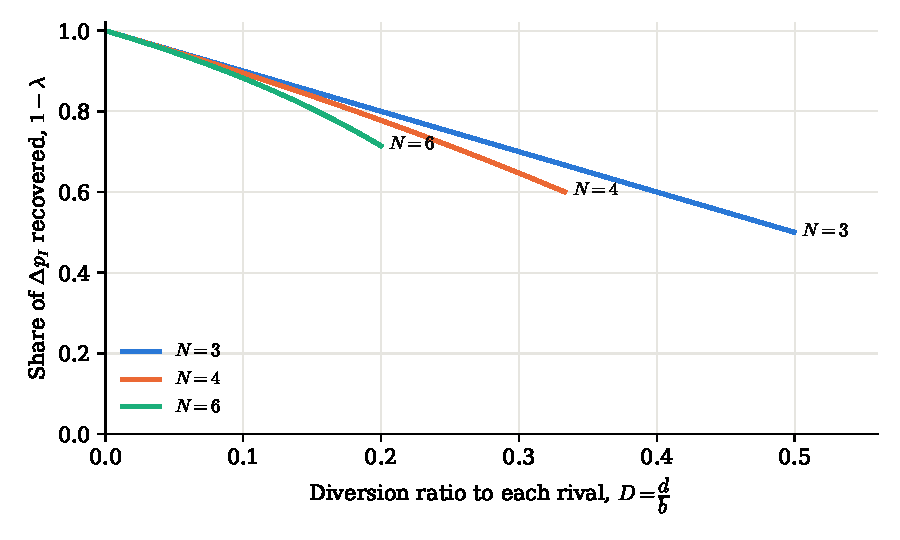
\includegraphics[width=0.78\textwidth]{figures/ch11/did_bias.pdf}
\caption{Share of the insiders' price increase recovered by a DiD estimator that uses an outsider as the control,
$1-\lambda$ from \eqref{eq:11-lambda}, against the diversion ratio to each rival $D=\frac{d}{b}$. Each curve
ends where $b=(N-1)d$. The bias is largest when the products are close substitutes, which is when the merger
matters most.}
\label{fig:11-didbias}
\end{figure}

\Cref{fig:11-didbias} shows the bias for several market sizes. Four lessons follow. First, a DiD that uses rival
brands as controls estimates a lower bound with the correct sign, which is how
\citet{AshenfelterHosken2010} and \citet{AshenfelterHoskenWeinberg2013} use it. Second, the bias grows with
diversion, so it is largest exactly when the merger has the largest effect. Third, a private-label control escapes
the bias only to the extent that store brands are distant substitutes supplied elastically. If store-brand prices
also rise, the bias has the same sign. Fourth, the rivals' price increase is itself an effect of the merger. Total
consumer harm includes it, and \cref{sec:11-dafny} shows how a study can be built on it.

\begin{remark}[General demand]\label{rem:11-didbias-general}
The linear form is not needed for the sign. Let $N=3$ and let $r(p_1,p_2)$ be the outsider's best response, with
partial derivatives $r_1,r_2>0$ (strategic complements) and $r_1+r_2<1$ (the usual stability condition). If the
symmetric insiders raise both prices by $\Delta p_I$, the mean value theorem gives
$\Delta p_O=(r_1+r_2)\big|_{\tilde p}\,\Delta p_I$ at some intermediate price vector $\tilde p$. Then
$0<\Delta p_O<\Delta p_I$. \citet{DeneckereDavidson1985} show for a broad class of demand systems that merging
firms raise prices by more than outsiders. How much outsiders respond depends on how fast elasticities change
with price \citep{CrookeEtAl1999}.
\end{remark}

\subsection{Event windows and transitory selection}\label{sec:11-retro-windows}

The \emph{event window} is the set of months used before and after the merger. It should be long enough to
capture the price change and short enough to avoid contamination by other events. \citet{AshenfelterHosken2010}
prefer a window that drops the three months before and after consummation and uses equal spans of data on the
two sides. Dropping the months near the merger avoids the question of exactly when the parties start pricing
jointly. The law prohibits joint pricing before closing, yet \citet{KimSingal1993} find that many airlines raised
fares before their mergers were consummated \citep[footnote~47]{AshenfelterHosken2008}. The symmetric design protects against a subtler
problem, which we now formalize following \citet{HeckmanRobb1985} and \citet{AshenfelterCard1985}.

Suppose that without the merger log prices follow $y_{jt}(0)=\alpha_j+\tau_t+u_{jt}$. Here $\tau_t$ is common to
all products and $u_{jt}$ is a transitory deviation. Mergers may be triggered by transitory events. A price war,
for example, depresses $u_{j t_0}$ and may push firms to merge. The General Mills purchase of the Chex brands was
announced just after a widely reported price war in ready-to-eat cereal in April 1996 \citep[p.~15]{AshenfelterHosken2008}.

\begin{definition}[Time reversibility]\label{def:11-reversible}
A stationary process $\{u_t\}$ is \emph{time reversible} if, for every $s\ge1$, the pairs $(u_{t_0+s},u_{t_0})$ and
$(u_{t_0-s},u_{t_0})$ have the same joint distribution.
\end{definition}

Every stationary Gaussian process is time reversible. Its joint distributions depend only on the autocovariance
function, and the autocovariance at lag $s$ equals the autocovariance at lag $-s$.

\begin{proposition}[Symmetric windows remove transitory selection]\label{prop:11-window}
Suppose $\{u_{jt}\}_t$ is stationary, time reversible and independent of $\alpha_j$. Suppose the event $A_j$ that
product $j$'s owner merges at $t_0$ depends only on $\alpha_j$, on $u_{jt_0}$ and on variables independent of the
process $\{u_{jt}\}$. Then for every $s\ge1$,
\begin{equation*}
\E\big[u_{j,t_0+s}-u_{j,t_0-s}\mid A_j\big]=0.
\end{equation*}
\end{proposition}

\begin{proof}
Condition first on $(\alpha_j,u_{jt_0})$ and use the law of iterated expectations:
\begin{equation*}
\E\big[u_{j,t_0+s}\mid A_j\big]=\E\Big[\E\big[u_{j,t_0+s}\mid \alpha_j,u_{jt_0}\big]\mid A_j\Big]
=\E\Big[\E\big[u_{j,t_0+s}\mid u_{jt_0}\big]\mid A_j\Big].
\end{equation*}
The second equality uses the independence of the process from $\alpha_j$ and from the other variables in $A_j$. By
time reversibility $\E[u_{j,t_0+s}\mid u_{jt_0}]=\E[u_{j,t_0-s}\mid u_{jt_0}]$. Applying the same two steps
in reverse gives $\E[u_{j,t_0-s}\mid A_j]$.
\end{proof}

The proposition implies that a comparison of month $t_0+s$ with month $t_0-s$ has no transitory selection bias.
So does any average of such comparisons over $s=k,\dots,K$. An asymmetric window does not have this property. Let
$u_{jt}$ be a Gaussian AR(1) process with coefficient $0.8$, and suppose mergers follow price wars, so that
$\E[u_{jt_0}\mid A_j]=-\mu<0$. Then $\E[u_{j,t_0\pm s}\mid A_j]=-(0.8)^{s}\mu$. Compare months 4 to 15 after
the merger with months 4 to 6 before it. The average post-merger deviation is $-0.159\mu$ and the average
pre-merger deviation is $-0.333\mu$. The estimate is biased upward by $0.174\mu$, because the recovery from the
price war is attributed to the merger. The symmetric window guards against this, at the cost of discarding data.
\citet{AshenfelterHosken2010} also report a symmetric window that keeps the months near the merger and an
asymmetric window that uses all available data. The window mattered little except for the cereal merger
\citep[p.~26]{AshenfelterHosken2008}.

Windows also determine which effects we measure. A short window captures the short-run price response. Cost
savings may take longer to reach prices. \citet{FocarelliPanetta2003} find that the price effects of the bank
mergers they study were reversed by efficiency gains after about three years. Long windows, on the other hand, mix the merger
with entry, new products and repositioning, which grow more important as time passes \citep[footnote~49]{AshenfelterHosken2008}.

\subsection{Measuring prices and drawing inferences}\label{sec:11-retro-measure}

\casehead{Unit values versus price indices} A brand is sold in several package sizes $k=1,\dots,K$ with prices per
unit $p_{kt}$ and unit sales $q_{kt}$. The \emph{unit value} or average revenue of the brand is
\begin{equation*}
P^{AR}_t=\frac{\sum_k p_{kt}q_{kt}}{\sum_k q_{kt}}=\sum_k\omega_{kt}\,p_{kt},\qquad \omega_{kt}=\frac{q_{kt}}{\sum_l q_{lt}}.
\end{equation*}
Its change between two periods decomposes as
\begin{equation*}
P^{AR}_1-P^{AR}_0=\sum_k\omega_{k0}\,(p_{k1}-p_{k0})+\sum_k(\omega_{k1}-\omega_{k0})\,p_{k1}.
\end{equation*}
The first term is a price change at fixed quantity weights. The second is a composition effect. If buyers shift
toward large packages, which are cheaper per unit, the unit value falls even when every package price rises. A
\emph{Stone price index} with fixed revenue weights $\bar w_k$ removes the composition term:
\begin{equation*}
\ln P^{S}_t=\sum_k\bar w_k\ln p_{kt},\qquad \ln P^{S}_1-\ln P^{S}_0=\sum_k\bar w_k\,(\ln p_{k1}-\ln p_{k0}).
\end{equation*}
\citet{AshenfelterHosken2010} construct five price measures for cereal, syrup and feminine hygiene products. They
are the unit value, two revenue-weighted average prices with first-year or last-year weights, and two Stone indices
with the same weights. They aggregate weekly data to months to dampen the effect of household stockpiling during sales
\citep{HendelNevo2006}. Scanner data also record retail prices. A merger of manufacturers changes wholesale
prices, and retail prices change by the retailers' pass-through of the wholesale change.

\casehead{Clustered errors} In \eqref{eq:11-ah-price} the regressor $\mathit{Post}_t$ takes the same value for
every product and region in a month. Common monthly shocks then make the errors of a month correlated, and
conventional standard errors are too small \citep{Moulton1987}.

\begin{lemma}[Moulton factor]\label{lem:11-moulton}
Let $y_{it}=\beta_0+\beta x_t+e_{it}$ for $i=1,\dots,m$ observations in each of $T$ months, with
$e_{it}=v_t+w_{it}$, where $v_t$ and $w_{it}$ are independent with mean zero and variances $\sigma_v^2$ and
$\sigma_w^2$. Let $\rho_e=\frac{\sigma_v^2}{\sigma_v^2+\sigma_w^2}$. Then the variance of the OLS estimator
$\hat\beta$ is $1+(m-1)\rho_e$ times the conventional formula that treats the errors as independent.
\end{lemma}

\Cref{lem:11-moulton} is the special case of \cref{prop:A-moulton} with months as clusters of size $m$. The error
components make the errors homoskedastic with variance $\sigma_v^2+\sigma_w^2$, independent across months and
equicorrelated within a month with correlation $\rho_e$. The regressor is constant within a month, so its
intra-cluster correlation is $\rho_x=1$. Then \eqref{eq:A-moulton} gives the factor $1+(m-1)\rho_e$.

With 64 regions and an intra-month correlation of only $0.1$, the factor is $7.3$, and the correct standard error
is $2.7$ times the conventional one. \citet{AshenfelterHosken2010} cluster by month. Clustering by month also
requires enough months, and serial correlation across months is a further concern in DiD designs
\citep{BertrandDufloMullainathan2004}.

\subsection{Which mergers can we study? Selection by the agencies}\label{sec:11-retro-select}

The agencies screen proposed mergers and block or modify those they expect to raise prices. As
\cref{sec:11-review} showed, about 97\% of the mergers filed from 1991 to 2004 went ahead without a full
investigation, and most of the rest were modified, abandoned or blocked. Retrospective samples therefore contain
only cleared mergers. A simple model shows what such samples can reveal.

\begin{assumption}[Screening on a noisy signal]\label{ass:11-screen}
Merger $m$ has a true price effect $\Delta_m$. The agency observes a signal $S_m=\Delta_m+\eta_m$ and clears the
merger if $S_m\le\bar s$. The pair $(\Delta_m,\eta_m)$ is jointly normal and independent across mergers, with
$\Delta_m$ of mean $\mu_\Delta$ and variance $V_\Delta>0$, and $\eta_m$ of mean zero and variance $V_\eta$,
independent of $\Delta_m$.
\end{assumption}

\begin{proposition}[What cleared mergers reveal]\label{prop:11-select}
Under \cref{ass:11-screen},
\begin{equation*}
\E[\Delta_m\mid S_m\le\bar s]\ \le\ \E[\Delta_m\mid S_m=\bar s]\ \le\ \E[\Delta_m\mid S_m>\bar s],
\end{equation*}
and $\E[\Delta_m\mid S_m\le\bar s]\le\mu_\Delta$, the average effect without enforcement.
\end{proposition}

\begin{proof}
Joint normality gives the linear conditional expectation
\begin{equation*}
\E[\Delta_m\mid S_m=s]=\mu_\Delta+k\,(s-\mu_\Delta),\qquad k=\frac{V_\Delta}{V_\Delta+V_\eta}\in(0,1],
\end{equation*}
which is increasing in $s$. Averaging an increasing function over $s\le\bar s$ gives at most its value at $\bar
s$, and averaging over $s>\bar s$ gives at least that value. Finally, $\mu_\Delta$ is a weighted average of the
cleared and blocked means, so it lies between them.
\end{proof}

A random sample of cleared mergers therefore gives a lower bound on the price effect of a typical merger in a
world without enforcement \citep{Carlton2009}. That bound says little about policy, because most proposed
mergers raise no competitive concern. The informative object is the effect of the \emph{marginal merger},
$\E[\Delta_m\mid S_m=\bar s]$. If it is positive, enforcement under a consumer-welfare standard is too lenient at
the margin. If it is negative, enforcement is too strict \citep{AshenfelterHoskenWeinberg2013}. Both studies below
target the margin. \citet{AshenfelterHosken2010} pick cleared mergers that look most problematic from public
information. Their estimates therefore bound from above the effects of other cleared mergers and from below the
effects of blocked ones. \citet{AshenfelterHoskenWeinberg2013} study a merger that was nearly challenged. Two caveats
apply. Researchers see public concentration measures, which are a noisy proxy for the agency's signal. And
samples are also selected by data availability, which favors consumer products and formerly regulated
industries such as airlines, banking and hospitals.

\subsection{Stock-market event studies}\label{sec:11-retro-event}

Before scanner data, retrospectives used stock prices. The method of abnormal returns is developed in
\cref{sec:A-eventstudy}, and \cref{sec:09-wc-method} applies it to airline entry. Its application to mergers, due to \citet{Eckbo1983} and \citet{Stillman1983}, looks at
the merging firms' \emph{rivals}. A merger that raises market power, through unilateral or coordinated effects,
raises rivals' profits. A merger that makes the merged firm a more efficient and tougher competitor lowers them.
News that raises the chance of the merger (the announcement) and news that lowers it (an antitrust complaint)
therefore move rivals' values in opposite directions under each hypothesis. \Cref{tab:11-eventpred} lists the
predictions.

\begin{table}[htbp]
\centering
\caption{Predicted abnormal returns of rival firms}
\label{tab:11-eventpred}
\footnotesize
\begin{tabular}{@{}lcc@{}}
\toprule
Hypothesis & Merger announcement & Antitrust complaint \\
\midrule
Market power (higher post-merger prices) & $+$ & $-$ \\
Efficiency (merged firm a tougher rival) & $-$ & $+$ \\
Information (merger reveals industry-wide gains) & $+$ & $0$ \\
\bottomrule
\end{tabular}

\smallskip
\begin{minipage}{0.85\linewidth}
\footnotesize Notes: Signs of rivals' cumulative abnormal returns. Under the information hypothesis the
announcement reveals profitable opportunities, such as scale economies or the value of rivals as future targets,
that a complaint against one merger does not withdraw.
\end{minipage}
\end{table}

\citet[p.~269]{Eckbo1983} studies the rivals of 65 challenged horizontal mergers. On average they earned an
abnormal return of 2.45 percent over the 31 days around the merger proposal, more than three standard deviations
from zero. Over the 31 days around the antitrust complaint their average return was 1.78 percent, about one standard
deviation from zero, so they did not lose. Eckbo concludes that the data generally reject the collusion hypothesis
(p.~242). He reads the rivals' gains at the proposal as news of cost savings that they can also achieve. He calls
this the productive efficiency hypothesis, which corresponds to the information row of \cref{tab:11-eventpred}.
\citet[p.~240]{Stillman1983} studies the rivals of 11
challenged horizontal mergers attempted between 1964 and 1972. Only in the merger of Sterling Drug and Lehn and Fink
did their returns broadly follow the market-power pattern. In nine of the 11 mergers the rivals showed no abnormal
returns of any kind.
These designs have known limits. Rival returns mix the three hypotheses. News may be anticipated, so the window
captures only part of it. Rivals are often diversified firms, and the affected market can be a small part of
their value. Many relevant rivals are not publicly traded. \citet{Woolley1989} applies the method to 29
merger-related events in hospital chains between 1969 and 1985. \citet{VitaSchumann1991} criticize his choice of
events and rivals and note that listed chains own a small share of hospitals (\citealp[p.~11]{Dafny2005}).
\citet{McAfeeWilliams1988} study the 1979 acquisition of Kalvar by Xidex, two producers of duplicate microfilm. The FTC
challenged the merger in September 1980 (p.~201). McAfee and Williams cite \citet{BartonSherman1984}, who find that
the ratio of vesicular to diazo prices paid by the federal government rose about 25 percent after the merger
\citep[p.~200]{McAfeeWilliams1988}.
An event study of the rivals' returns nevertheless shows no evidence of harm (pp.~202--203).
\citet[p.~231, n.~137]{AskerNocke2021} reach a similar verdict on the literature that runs from \citet{Eckbo1983}
and \citet{Stillman1983} to \citet{DusoNevenRoller2007}. Most authors in it are cautious about what an event study
reveals about the competitive effects of a particular merger. In the words of \citet{KaplowShapiro2007}, an event
study ``measures the expectations of investors about merger effects, not the actual effects of mergers.'' The method
has worked best for patterns across large samples of mergers, as in \citet{DusoNevenRoller2007}. For these reasons
modern retrospectives measure prices directly.

\subsection{Five consumer-product mergers: Ashenfelter and Hosken (2010)}\label{sec:11-ah}

\casehead{Question and design} \citet{AshenfelterHosken2010} ask whether the mergers that the agencies let through
raised consumer prices.\footnote{We use the NBER working-paper version \citep{AshenfelterHosken2008}. Table
numbers and page references follow it.} Their design follows \cref{prop:11-select}. They search the Merger
Yearbook for consummated mergers in consumer-product industries between 1997 and 1999 whose parties sold
substitutes in concentrated markets. The period is fixed by the data, because the vendor sold scanner data only
for the previous five years. Three of the five selected mergers went through without government action:
Procter and Gamble's purchase of Tambrands, Aurora Foods' purchase of Kraft's Log Cabin syrup, and Pennzoil's
purchase of Quaker State. Two were modified by the FTC: General Mills' purchase of Ralcorp's branded cereals and
the merger of Guinness and Grand Metropolitan into Diageo. All five produced highly concentrated markets (HHI above
1,800) with HHI increases above 100 points, the 1992 Guidelines' presumption of harm.

The authors argue that these mergers sit near the enforcement margin. In the FTC's investigations of fiscal years
1996--2003, 46\% of markets had post-merger HHI below 3,000 and 51\% had increases below 800 points. All five
mergers have post-merger HHIs below 3,000 and HHI changes between 200 and 1,000 points, so they sit near the median
of the investigated markets (p.~12). The FTC acted in 25\% of investigated markets with post-merger HHI below 2,500
(four of the five mergers) and in 44\% of markets with increases below 800 (pp.~11--12).

\casehead{The five mergers} Procter and Gamble bought Tambrands for \$1.85 billion in July 1997, adding the leading
tampon (Tampax) to the leading sanitary pad (Always). The Justice Department reviewed the deal and took no
action. Guinness and Grand Metropolitan combined their spirits portfolios in a transaction valued at about \$36
billion. The FTC found harm in premium scotch and premium gin and required the sale of the Bombay gins and Dewar's
scotch to Bacardi for \$1.9 billion. Pennzoil bought Quaker State for \$1 billion in December 1998, combining two
of the five premium motor-oil brands. General Mills bought the Chex cereals for \$570 million in January 1997.
Ralcorp kept its private-label business, the largest in the country, and the FTC's modifications let Ralcorp make
private-label Chex at once. Aurora, owner of Mrs.\ Butterworth's, bought Log Cabin for \$222 million in July 1997,
joining two of the three major syrup brands (pp.~12--16). \Cref{tab:11-ah} reports shares and concentration,
and \cref{tab:11-ahhhi} in \cref{sec:11-hhi} checked the reported changes in concentration against $2s_As_B$.

\begin{table}[htbp]
\centering
\caption{Five consumer-product mergers: concentration and aggregate price effects}
\label{tab:11-ah}
\footnotesize
\begin{tabular}{@{}lcccccc@{}}
\toprule
& & & & & \multicolumn{2}{c}{Aggregate price effect} \\
\cmidrule(l){6-7}
Transaction (industry) & Shares (\%) & HHI & $\Delta$HHI & & Private label & Branded \\
\midrule
General Mills / Ralcorp (cereal) & 28, 4 & 2,357 & 238 & & 0.032 & 0.057 \\
 & & & & & (0.005) & (0.005) \\
Pennzoil / Quaker State (motor oil) & 29, 9 & 2,189 & 517 & & 0.052 & 0.014 \\
 & & & & & (0.013) & (0.011) \\
P\&G / Tambrands (feminine protection) & 25, 19 & 2,815 & 959 & & 0.070 & 0.023 \\
 & & & & & (0.008) & (0.007) \\
Aurora / Log Cabin (pancake syrup) & 15, 19 & 1,990 & 589 & & 0.004 & 0.012 \\
 & & & & & (0.011) & (0.005) \\
Guinness / Grand Met (liquor), overall & 21, 22 & 2,026 & 935 & & 0.027 & $-0.010$ \\
 & & & & & (0.003) & (0.003) \\
\quad gin & & & & & 0.022 & $-0.021$ \\
 & & & & & (0.005) & (0.003) \\
\quad scotch & & & & & 0.071 & 0.031 \\
 & & & & & (0.006) & (0.002) \\
\quad vodka & & & & & 0.011 & $-0.021$ \\
 & & & & & (0.003) & (0.005) \\
\bottomrule
\end{tabular}

\smallskip
\begin{minipage}{0.97\linewidth}
\footnotesize Notes: Shares are pre-merger revenue shares of the acquirer and the target, in that order (for syrup,
Aurora then Philip Morris's Log Cabin). HHI is the post-merger HHI and $\Delta$HHI its change, from pre-merger
revenue data, with private labels treated as one participant. Price effects are the revenue-weighted averages
\eqref{eq:11-ah-agg} of the product-level estimates of $\beta_2$ in \eqref{eq:11-ah-price}, using the private-label
or the branded control group. Standard errors in parentheses assume zero covariances among the components. The data come from IRI's food channel (64 regions) for
cereal, feminine protection and syrup, its mass-merchandiser channel (10 regions) for motor oil, and its drug-store
channel (5 regions) for liquor. Source: \citet{AshenfelterHosken2008}, Tables 2 and 13.
\end{minipage}
\end{table}

\casehead{Data} The data are weekly revenue and unit sales by Universal Product Code (UPC), purchased from
Information Resources Inc.\ (IRI) and aggregated to months. IRI projects sales for each channel and metropolitan
area from a sample of stores. The authors choose for each merger the channel that best represents consumer
purchases. Food products use the food channel in 64 InfoScan markets. Motor oil uses the mass-merchandiser channel
in 10 markets, because consumers who change their own oil buy it there. Liquor uses the only available source, a
drug-store sample with complete data for five markets in three states. The markets are San Francisco, San Diego,
Los Angeles, Chicago and Phoenix, which limits external validity (pp.~16--18). Motor oil is priced as revenue per quart for
each brand and weight. Spirits are priced separately for the 750 ml and 1.75 litre bottles. The other categories
use the five price measures of \cref{sec:11-retro-measure}.

\casehead{Estimation} The price equation \eqref{eq:11-ah-price} is fitted by OLS separately for each merging
product, with standard errors clustered by month. The preferred specification uses the unit value, the symmetric
window that drops three months on each side, and one of two control groups. The \emph{private-label control} uses
the store brands closest to each merging product. These are private-label motor oil, feminine hygiene products and
maple-flavored syrup, private-label gin, scotch and vodka for the spirits, and private-label cereals in the same
IRI segments for cereal. The \emph{branded control} uses close branded substitutes, such as the three other premium motor oils
(Havoline, Valvoline and Castrol). The authors treat the branded estimates mainly as a specification check, for the
reason given in \cref{prop:11-didbias} (pp.~23--24). They also report regressions with no control group.

\casehead{Results} \Cref{tab:11-ah} gives the aggregate effects (Table 13). With the private-label control, four of
the five mergers raised prices by roughly 3\% to 7\%. The estimates are 3.2 log points for General Mills and Chex,
5.2 for Pennzoil and Quaker State, 7.0 for Procter and Gamble and Tambrands, and 2.7 for Diageo. The syrup merger had no
detectable effect (0.4). The branded control gives larger effects for cereal and syrup and smaller ones for the
other three. The spirits merger illustrates the role of the control group. Scotch prices rose under both controls
(7.1 and 3.1 log points), while gin and vodka rose relative to private labels and fell relative to branded
rivals.

The product-level estimates show that the merged firms did not raise all prices together. \Cref{tab:11-ah-pqs}
reproduces Table 3 for motor oil. Relative to private labels, Quaker State rose 8.1 log points and Quaker State
Deluxe 6.1, while the much larger Pennzoil brand rose 3.9. In Table 3, Quaker State's increase ranks first among
the 12 products compared, its own and the 11 branded controls. The text instead describes it as larger than all but
one control brand (p.~28). Market shares moved accordingly. Quaker State lost 1.31 points of revenue share, 13.6\%
of its pre-merger share, while Pennzoil gained 4.22 points. Because Pennzoil's gain exceeded Quaker State's loss,
it grew at the expense of rivals as well. The authors read this as a strategy of raising the price to customers
loyal to Quaker State while holding the price of the larger brand (p.~29).

\begin{table}[htbp]
\centering
\caption{Pennzoil and Quaker State: product-level price and share effects}
\label{tab:11-ah-pqs}
\footnotesize
\begin{tabular}{@{}lcccccc@{}}
\toprule
& \multicolumn{2}{c}{Price effect $\hat\beta_2$} & \multicolumn{2}{c}{Rank in control group} &
\multicolumn{2}{c}{Change in revenue share} \\
\cmidrule(lr){2-3}\cmidrule(lr){4-5}\cmidrule(l){6-7}
Product & Branded & Private label & Branded & Private label & Points & Percent \\
\midrule
Pennzoil & 0.004 & 0.039 & 8/12 & 1/2 & 4.22 & 18.47 \\
 & (0.015) & (0.019) & & & (0.83) & \\
Quaker State & 0.035 & 0.081 & 1/12 & 1/2 & $-1.31$ & $-13.58$ \\
 & (0.016) & (0.015) & & & (0.47) & \\
Quaker State Deluxe & 0.021 & 0.061 & 4/12 & 1/2 & $-0.16$ & $-5.95$ \\
 & (0.021) & (0.022) & & & (0.13) & \\
\bottomrule
\end{tabular}

\smallskip
\begin{minipage}{0.95\linewidth}
\footnotesize Notes: Standard errors in parentheses. The rank orders the product's estimated price change among
the control products in descending order: 8/12 means that seven control products had larger increases. Quantity
shares move similarly ($+4.46$, $-1.32$ and $-0.13$ points). Monthly data from 10 regions of IRI's
mass-merchandiser channel, January 1997 to December 2000, excluding October 1998 to March 1999. An observation is
a product, city and month. The regressions have about 9,000 (branded control) and 2,000 (private-label control)
observations. Source: \citet{AshenfelterHosken2008}, Table 3.
\end{minipage}
\end{table}

The other mergers show the same selectivity (Tables 5, 7, 9 and 11). After buying Tambrands, Procter and Gamble
raised the prices of Always liners and pads by 8.0 and 7.8 log points relative to store brands, and Tampax by
5.8.
Relative to branded products the liner and pad increases were 6.1 and 4.5, and Tampax fell by 0.9. A later study
of the same merger, \citet{Weinberg2011}, reports increases of 8 percent for Always pads and 5 percent for Tampax
relative to private label \citep[p.~262]{AskerNocke2021}. General
Mills left the Chex prices almost unchanged (at most 0.8 log points under either control) and raised the prices
of its own Cheerios and Wheaties brands. Cheerios rose 4.4 log points relative to store brands and 4.6 relative
to branded cereals. Every scotch product rose relative to its private-label control, by 5.5 to 9.8 log points.
For syrup, Log Cabin's 2.8 log point rise relative to branded syrups was not robust, and Mrs.\ Butterworth's prices
did not change.

\casehead{Robustness} For each merger, a summary table pools the estimates across windows, price measures and
control groups (Tables 4, 6, 8, 10 and 12). For motor oil, all 18 estimates are positive. All nine private-label
estimates have $t$-statistics above two, against three of the nine branded estimates. For feminine protection,
92\% of the private-label estimates and 78\% of the branded ones are positive. About 90\% of the cereal estimates
are positive, and none of the negative ones is below $-1\%$. For syrup, about two thirds fall between $-1\%$ and
$+1\%$. The choice of window mattered little except for cereal. The price measure left the signs unchanged and
changed the magnitudes. With weekly data the cereal estimates depended heavily on the price measure, which points to
stockpiling and package substitution (pp.~26--32). Regressions with no control group also show price increases
after virtually every merger (Appendix Tables 3--7). For example, the no-control estimates for Quaker State and
Always pads are 0.061 (0.016) and 0.053 (0.003).

\casehead{Comparison with a merger simulation} The General Mills and Chex merger had been simulated by
\citet{Nevo2000b} with a random-coefficients demand model (\cref{sec:11-simulation}). As cited by Ashenfelter and
Hosken, the published simulation predicts increases before efficiencies of 12.2\% for Chex, 1.1\% for Cheerios,
0.8\% for Honey Nut Cheerios and 0.1\% for Wheaties (p.~32). The retrospective finds the opposite pattern: little
change for Chex and increases for the General Mills brands. Possible reasons include the different data
(quarterly data for 1988--1992 in the simulation), new product introductions, and the demand specification. The
consent decree's provision for private-label Chex may also have restrained Chex pricing, an entry threat that a
simulation with a fixed set of products cannot represent (footnote 60).

\casehead{Interpretation and limitations} The best estimate of the price effect of mergers near the enforcement
margin is positive and modest. This finding cuts against both camps in the enforcement debate. Advocates of less
intervention expect the marginal merger to lower prices through efficiencies, and advocates of more intervention
expect large increases (p.~35). The authors list three limitations themselves (p.~36). Consumer-product mergers are a
small part of all mergers: 20 percent of the 8,013 filings in 1997 and 1998 shared the studied firms' two-digit
industry codes. The design cannot capture longer-run efficiency effects or new products. Finally, the study examines
only one kind of enforcement error, the failure to block harmful mergers, and leaves aside the blocking or
deterrence of benign ones. Several further points deserve attention. The selection rests on public concentration measures, which
may misjudge which mergers the agencies found marginal. The private-label control may itself be a substitute,
especially in cereal, where Ralcorp kept a large store-brand business. The aggregate standard errors ignore
covariances, as shown after \eqref{eq:11-ah-agg}. Retail scanner prices measure the merger's effect after
retailers' pass-through. Finally, the results vary across products within a merger, so several products and
specifications are tested for each merger, and some significant estimates will arise by chance.

\casehead{Contribution} The paper turned merger retrospectives into a program-evaluation exercise with explicit
attention to control groups, windows, price measurement and the selection of mergers. It shows that a cleared
merger's effect can be concentrated on a few products, and it supplied the retrospective benchmarks later used to
grade merger simulations.

\subsection{A nearly blocked merger of appliance makers: Ashenfelter, Hosken and Weinberg (2013)}\label{sec:11-maytag}

\casehead{Question} \citet{AshenfelterHoskenWeinberg2013} estimate the price effects of Whirlpool's acquisition of
Maytag.\footnote{We use the NBER working-paper version \citep{AshenfelterHoskenWeinberg2011}. Table numbers
follow it and may differ from the published article.} The merger is a natural candidate for the marginal merger
of \cref{prop:11-select}. Commentators argued that the Justice Department would have challenged it a decade
earlier, and the decision not to act came to symbolize lenient enforcement \citep{BakerShapiro2008}.

\casehead{Background} In mid-2005 a group of private investors agreed to buy Maytag for \$1.13 billion. The Haier
Group, a Chinese appliance maker with little presence in the United States, then offered \$1.3 billion. Whirlpool,
the largest United States manufacturer, offered \$1.4 billion on July 17, and Haier withdrew three days later.
Whirlpool bought Maytag for \$1.79 billion on March 30, 2006, after a long Justice Department investigation. The
merger reduced the major appliance manufacturers from four (Whirlpool, Maytag, GE and Electrolux) to three. The
Justice Department's closing statement of March 29, 2006, focused on washers and dryers and gave three reasons for
not acting. GE and Electrolux had excess capacity, and the recent entrants LG and Samsung could expand imports.
Large retailers had alternatives to resist price increases. The parties had substantiated large cost savings
(printed pp.~4--6 and 21).

\casehead{Market structure} \Cref{tab:11-maytag} reproduces the pre-merger revenue shares. Whirlpool was the
largest firm in dishwashers, dryers, refrigerators and washers, with 39\% to 49\% of revenue, and Maytag held 9\%
to 17\%. The increase in the HHI matches $2s_Ws_M$ in every category up to rounding of the
shares, within three points. In dryers, for example, $2\times48.8\times16.6=1{,}620$. The parties overlapped less in
cooktops, freezers, ovens and ranges. Neither had more than 1 percent of freezer revenue, Maytag held 5 to 10 percent
of the other three, and the implied HHI changes were 256 to 416 points.
These four categories serve as comparison groups, restricted to brands not made by Whirlpool or Maytag.

\begin{table}[htbp]
\centering
\caption{Whirlpool and Maytag: pre-merger revenue shares and concentration}
\label{tab:11-maytag}
\footnotesize
\begin{tabular}{@{}lccccc@{}}
\toprule
Category & Whirlpool & Maytag & Largest rivals & HHI & $\Delta$HHI \\
\midrule
\multicolumn{6}{@{}l}{\textit{Treated categories}} \\
Dishwashers & 38.6 & 11.4 & Electrolux 25.1, GE 12.5 & 2,453 & 880 \\
Clothes dryers & 48.8 & 16.6 & GE 12.2, LG 9.6, Electrolux 8.9 & 2,983 & 1,620 \\
Refrigerators & 41.8 & 9.2 & Electrolux 24.1, GE 10.9 & 2,595 & 770 \\
Clothes washers & 44.0 & 16.8 & Electrolux 13.8, GE 10.5, LG 10.2 & 2,632 & 1,478 \\
\addlinespace
\multicolumn{6}{@{}l}{\textit{Comparison categories}} \\
Cooktops & 22.0 & 9.5 & GE 20.8, Electrolux 19.1 & 1,571 & 416 \\
Freezers & $<1$ & $<1$ & Electrolux 81.3, Haier 12.8 & 6,789 & 0 \\
Ovens & 32.5 & 6.3 & GE 23.1, Electrolux 10.5 & 1,929 & 412 \\
Ranges & 24.7 & 5.2 & Electrolux 37.6, GE 25.3 & 2,703 & 256 \\
\bottomrule
\end{tabular}

\smallskip
\begin{minipage}{0.95\linewidth}
\footnotesize Notes: Revenue shares in percent from NPD data before the merger. HHI is the pre-merger HHI as
labelled in the source. Neither party had more than 1\% of freezer revenue before the merger. Kenmore, sold by
Sears and partly made by Whirlpool, is not in the data. Source: \citet{AshenfelterHoskenWeinberg2011}, Tables 1
and 2.
\end{minipage}
\end{table}

\casehead{Data} The NPD Group supplied national monthly unit sales and revenue for each appliance model, identified
by its stock-keeping unit (SKU), from January 2005 to September 2008. More than 14,000 SKUs enter during the
period, and observed characteristics explain 85\% to 95\% of the variation in prices. Two features of the industry
shape the design. First, most appliances have a life cycle of about a year. The authors estimate age profiles
separately for each category,
\begin{align}
\ln p_{jt}&=\alpha_j+\sum_{k=2}^{25}\theta_k\,\mathit{Age}_{kjt}+\sum_{l=2}^{43}\delta_l\,\mathit{Month}_{lt}+e_{jt},\label{eq:11-ahw-age}\\
\ln q_{jt}&=\psi_j+\sum_{k=3}^{25}\lambda_k\,\mathit{Age}_{kjt}+\sum_{l=3}^{43}\gamma_l\,\mathit{Month}_{lt}+u_{jt},\nonumber
\end{align}
where $\mathit{Age}_{kjt}$ indicates that model $j$ is $k$ months old.\footnote{In this subsection $\theta_k$,
$\delta_l$, $\psi_j$, $\lambda_k$ and $\gamma_l$ are regression coefficients with no relation to their meanings
elsewhere in the book.} Prices of washers, dryers, dishwashers, refrigerators, freezers and ranges typically fall by more
than 10\% after a year, and monthly sales fall by about half. Ovens and cooktops show no such decline. The analysis
therefore uses each model's first year only and controls for age by category. Second, many SKUs sell very few
units. The sample keeps models with at least 1,000 units in their first 13 months (100 for freezers, ovens and
cooktops). The retained models account for 90\% to 99\% of sales in the large categories (printed pp.~6--9).

\casehead{Estimating equations} The baseline specification, fitted by OLS separately for each treated and
comparison pair of categories, is
\begin{multline}\label{eq:11-ahw-fe}
\ln p_{jt}=\beta_1\,\mathit{Maytag}_j\,\mathit{Post}_t+\beta_2\,\mathit{Whirlpool}_j\,\mathit{Post}_t\\
+\sum_{k=3}^{13}\theta_k^{T}\mathit{Age}^{T}_{kjt}+\sum_{k=3}^{13}\theta_k^{C}\mathit{Age}^{C}_{kjt}+\sum_{l=2}^{43}\delta_l\,\mathit{Month}_{lt}+\alpha_j+e_{jt}.
\end{multline}
It has separate age profiles for the treated ($T$) and comparison ($C$) categories, month effects and SKU fixed
effects $\alpha_j$. The SKU fixed effects have a cost. The interactions are collinear with $\alpha_j$ for any model
sold only before or only after the merger. Equation \eqref{eq:11-ahw-fe} therefore identifies the effects only from
models sold on both sides of the merger date. With one-year life cycles, these are old models, and the merged firm may have
treated them differently from new ones. The authors therefore replace the fixed effects with observed
characteristics and brand dummies, such as a stainless-steel indicator, size, capacity and cycles:
\begin{multline}\label{eq:11-ahw-char}
\ln p_{jt}=x^{T}_{j}\beta^{T}+x^{C}_{j}\beta^{C}+\sum_{l=2}^{43}\delta^{C}_l\,\mathit{Month}_{lt}+\beta_1\,\mathit{Maytag}_j\,\mathit{Post}_t+\beta_2\,\mathit{Whirlpool}_j\,\mathit{Post}_t\\
+\sum_{k=3}^{13}\theta_k^{T}\mathit{Age}^{T}_{kjt}+\sum_{k=3}^{13}\theta_k^{C}\mathit{Age}^{C}_{kjt}+e_{jt}.
\end{multline}
Here $x^T_j$ is non-zero only for the parties' models and $x^C_j$ only for comparison models. Standard errors
are clustered by SKU. The check on this substitution is direct. On models sold both before and after the merger,
the two specifications give estimates within 0.2 percentage points of each other against cooktops and ranges.
Against cooktops, for instance, the Whirlpool dishwasher effect is 0.0432 with fixed effects and 0.0415 with
characteristics (Appendix Table 1). The gaps reach 0.7 points against ovens and 1 to 2 points against freezers, well
within one standard error (Appendix Tables 2--4).

The main specification splits each interaction by whether the model was introduced before (Old) or after (New)
the merger, which adds 35\% to 57\% to the sample. A within-category variant compares the parties' models with
rivals' models in the same category,
\begin{multline}\label{eq:11-ahw-rival}
\ln p_{jt}=x_j\beta+\sum_{k}\theta_k\,\mathit{Age}_{kjt}+\sum_{l}\delta_l\,\mathit{Month}_{lt}
+\beta_1\,\mathit{Maytag}_j\mathit{Post}_t\mathit{Old}_j+\beta_2\,\mathit{Whirlpool}_j\mathit{Post}_t\mathit{Old}_j\\
+\beta_3\,\mathit{Maytag}_j\mathit{Post}_t\mathit{New}_j+\beta_4\,\mathit{Whirlpool}_j\mathit{Post}_t\mathit{New}_j+e_{jt}.
\end{multline}
By \cref{prop:11-didbias}, the rival comparison is biased toward zero if rivals' models are substitutes.
Finally, product variety is measured by the number of SKUs selling at least 100 units a month,
\begin{equation}\label{eq:11-ahw-sku}
\ln\mathit{SKU}_{ft}=a+b\,\mathit{WM}_f+g\,\mathit{Post}_t+\delta^{V}\,\mathit{WM}_f\,\mathit{Post}_t+e_{ft},
\end{equation}
where $f$ is either the merged firm ($\mathit{WM}_f=1$) or all rivals together. The coefficient $\delta^V$ is the
proportional change in the merged firm's product count relative to rivals.

\casehead{Identification} The comparison categories identify the counterfactual price path. The design assumes that
cooktops, freezers, ovens and ranges made by other firms would have followed the same age- and
characteristic-adjusted price trend as the treated categories. All are durable goods bought with new homes and
remodeling, so they share much of the demand shock from the housing market. The data are national, so there is no
geographic variation. Identification rests entirely on comparisons across categories and, in
\eqref{eq:11-ahw-rival}, across firms within a category.

\begin{figure}[htbp]
\centering
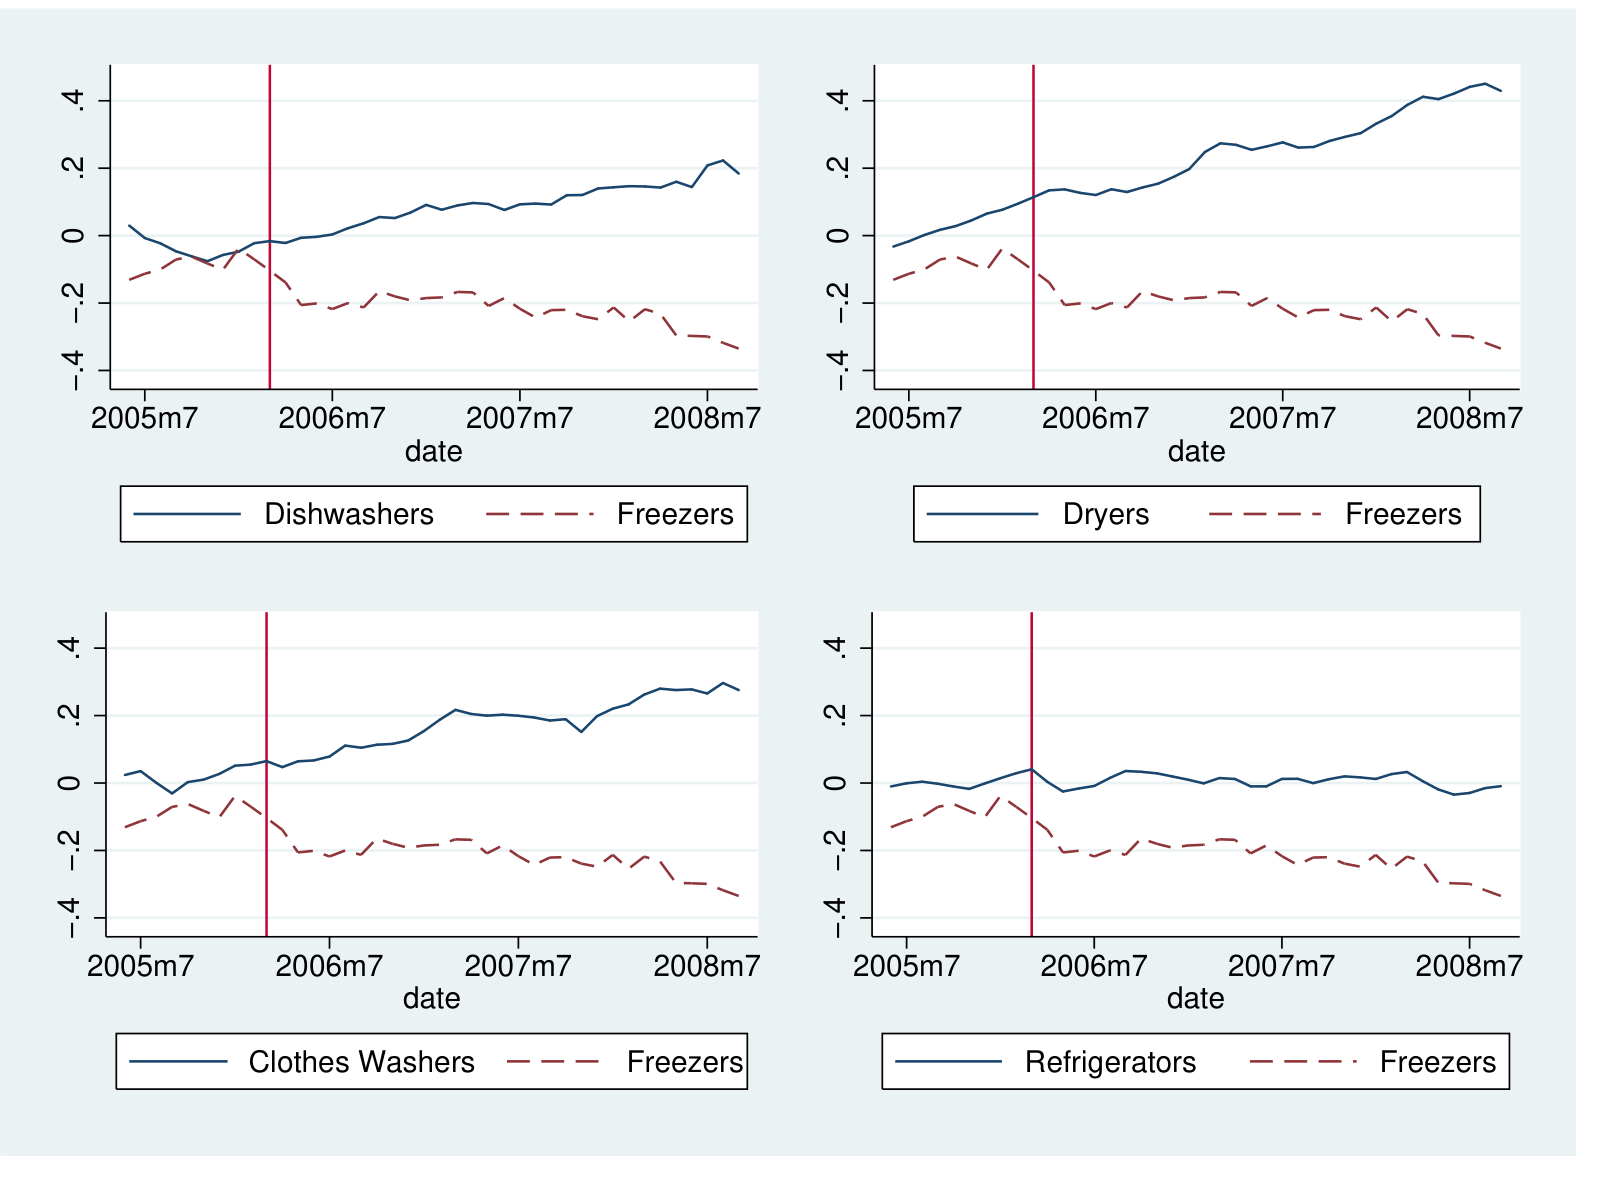
\includegraphics[width=0.86\textwidth]{figures/ch11/ahw_fig5.png}
\caption{Average log prices of Whirlpool and Maytag appliances (solid) and of freezers (dashed), adjusted for
product characteristics and age, May 2005 to September 2008. The vertical line marks consummation (March 30,
2006). Dishwasher, dryer and washer prices rise relative to freezers after the merger. Refrigerator prices do not.
The averages pool old and new models. The vintage-split regressions of \cref{tab:11-maytag-res} find no increase for
new washers. Source: \citet{AshenfelterHoskenWeinberg2011}, Figure 5.}
\label{fig:11-maytag}
\end{figure}

\casehead{Results} \Cref{fig:11-maytag} plots adjusted prices against freezers. \Cref{tab:11-maytag-res} reproduces
the regression estimates for the four treated categories against each comparison category (Tables 3 to 6) and
against rivals in the same category (Table 7). The clearest effects are for models introduced after the merger.
New Whirlpool dryers rose by 13.3 to 17.1 log points relative to the comparison categories, all significant. New
Maytag dishwashers rose by 4.8 to 7.4 log points, all significant at 5\%. New Whirlpool refrigerators rose by 1.9 to
3.9 log points, significant except against freezers. The authors give this result little weight. They describe ``a
small price increase, 2-4\%, for Whirlpool refrigerators'' that is ``imprecisely estimated and not as robust as the
findings for clothes dryers or dishwashers'' (printed pp.~15--16). The within-category estimate is only 0.008
(0.009), and their abstract concludes that there were ``no price effects for refrigerators or clothes washers''
(PDF p.~1). \citet[p.~262]{AskerNocke2021} quote the same sentence from the published abstract. Washers show no
increase. New Whirlpool washers in fact fell
by 1.5 to 4.1 log points. Estimates for models introduced before the merger depend on the comparison category.
They tend to be positive against cooktops and freezers and smaller or negative against ovens and ranges. The
within-category comparison tells the same story: new Maytag dishwashers rose 8.2 log points and new Whirlpool
dryers 7.3 log points relative to rivals' new models.

\begin{table}[htbp]
\centering
\caption{Whirlpool and Maytag: price effects by category, model vintage and comparison group}
\label{tab:11-maytag-res}
\footnotesize
\begin{tabular}{@{}lccccc@{}}
\toprule
& \multicolumn{4}{c}{Comparison category, \eqref{eq:11-ahw-char} split by vintage} & Rivals, \eqref{eq:11-ahw-rival} \\
\cmidrule(lr){2-5}\cmidrule(l){6-6}
Post-merger $\times$ & Cooktops & Freezers & Ovens & Ranges & Same category \\
\midrule
\multicolumn{6}{@{}l}{\textit{Clothes dryers}} \\
Old $\times$ Whirlpool & $-0.0172$ & 0.0291 & $-0.0654$ & $-0.0602$ & $-0.055$ \\
 & (0.0198) & (0.0347) & (0.0218) & (0.0176) & (0.018) \\
Old $\times$ Maytag & 0.0437 & 0.0903 & $-0.0102$ & 0.000473 & 0.008 \\
 & (0.0132) & (0.0310) & (0.0153) & (0.00671) & (0.008) \\
New $\times$ Whirlpool & 0.133 & 0.140 & 0.171 & 0.144 & 0.073 \\
 & (0.0653) & (0.0479) & (0.0471) & (0.0542) & (0.030) \\
New $\times$ Maytag & 0.00486 & 0.0113 & 0.0574 & 0.0318 & $-0.002$ \\
 & (0.0864) & (0.0622) & (0.0623) & (0.0757) & (0.040) \\
Observations & 2,657 & 2,206 & 2,563 & 4,429 & 3,088 \\
\addlinespace
\multicolumn{6}{@{}l}{\textit{Dishwashers}} \\
Old $\times$ Whirlpool & 0.0325 & 0.0855 & $-0.00769$ & 0.0124 & 0.024 \\
 & (0.0135) & (0.0307) & (0.0168) & (0.00739) & (0.008) \\
Old $\times$ Maytag & 0.0275 & 0.0826 & $-0.00919$ & 0.0100 & 0.030 \\
 & (0.0161) & (0.0310) & (0.0188) & (0.0107) & (0.011) \\
New $\times$ Whirlpool & $-0.00127$ & $-0.0160$ & 0.00463 & 0.00115 & 0.014 \\
 & (0.0157) & (0.0161) & (0.0151) & (0.00684) & (0.007) \\
New $\times$ Maytag & 0.0662 & 0.0480 & 0.0711 & 0.0743 & 0.082 \\
 & (0.0206) & (0.0200) & (0.0200) & (0.0163) & (0.015) \\
Observations & 2,296 & 1,845 & 2,202 & 4,068 & 2,895 \\
\addlinespace
\multicolumn{6}{@{}l}{\textit{Refrigerators}} \\
Old $\times$ Whirlpool & $-0.0213$ & 0.0455 & $-0.0465$ & $-0.0221$ & $-0.044$ \\
 & (0.0227) & (0.0341) & (0.0240) & (0.0202) & (0.021) \\
Old $\times$ Maytag & $-0.0266$ & 0.0370 & $-0.0506$ & $-0.0254$ & $-0.045$ \\
 & (0.0267) & (0.0363) & (0.0286) & (0.0251) & (0.025) \\
New $\times$ Whirlpool & 0.0388 & 0.0194 & 0.0389 & 0.0210 & 0.008 \\
 & (0.0159) & (0.0164) & (0.0145) & (0.00951) & (0.009) \\
New $\times$ Maytag & 0.00602 & $-0.00641$ & 0.0157 & 0.00960 & $-0.026$ \\
 & (0.0212) & (0.0229) & (0.0200) & (0.0164) & (0.017) \\
Observations & 3,534 & 3,083 & 3,440 & 5,306 & 5,902 \\
\addlinespace
\multicolumn{6}{@{}l}{\textit{Clothes washers}} \\
Old $\times$ Whirlpool & $-0.00856$ & 0.0341 & $-0.0556$ & $-0.0431$ & $-0.040$ \\
 & (0.0256) & (0.0373) & (0.0273) & (0.0231) & (0.027) \\
Old $\times$ Maytag & 0.0383 & 0.0848 & $-0.0117$ & 0.00310 & 0.006 \\
 & (0.0177) & (0.0318) & (0.0195) & (0.0127) & (0.017) \\
New $\times$ Whirlpool & $-0.0175$ & $-0.0409$ & $-0.0150$ & $-0.0202$ & $-0.047$ \\
 & (0.0171) & (0.0175) & (0.0176) & (0.0106) & (0.013) \\
New $\times$ Maytag & 0.0157 & $-0.00743$ & 0.0223 & 0.0171 & $-0.014$ \\
 & (0.0179) & (0.0179) & (0.0180) & (0.0111) & (0.014) \\
Observations & 2,264 & 1,813 & 2,170 & 4,036 & 2,456 \\
\bottomrule
\end{tabular}

\smallskip
\begin{minipage}{0.97\linewidth}
\footnotesize Notes: OLS estimates of the post-merger change in log price of the parties' models, standard errors
in parentheses, clustered by SKU. Each row label is interacted with the post-merger indicator. Old (New) marks
models introduced before (after) the merger. Product characteristics, age dummies and month dummies are included
throughout. Coefficients are as printed in the source. Monthly NPD data, April 2005 to September 2008. Source:
\citet{AshenfelterHoskenWeinberg2011}, Tables 3 to 7.
\end{minipage}
\end{table}

\casehead{Market shares and variety} \Cref{tab:11-maytag-var} reproduces Table 8. The merged firm's revenue share
fell significantly in every treated category, by 4.6 points in dishwashers, 9.5 in dryers, 8.6 in refrigerators
and 7.3 in washers. The fall is consistent with the price increases in dryers and dishwashers. It also occurred in
refrigerators and washers, where prices did not rise, so it cannot be due to price alone. The merged firm cut its
product line. The number of high-volume Whirlpool and Maytag SKUs fell by about 10 a month in dryers and washers
and by about 12 in refrigerators. Relative to rivals, who expanded their lines, the merged firm's count fell by 22
to 53 log points.

\begin{table}[htbp]
\centering
\caption{Whirlpool and Maytag: market shares and product offerings after the merger}
\label{tab:11-maytag-var}
\footnotesize
\begin{tabular}{@{}lcccc@{}}
\toprule
& \multicolumn{2}{c}{Change in share} & Absolute change & Relative change \\
\cmidrule(lr){2-3}
Category & Revenue & Volume & in SKUs offered & in SKUs offered, $\delta^V$ \\
\midrule
Dishwashers & $-0.046$ (0.010) & $-0.043$ (0.011) & $-1.067$ (1.862) & $-0.219$ (0.044) \\
Clothes dryers & $-0.095$ (0.009) & $-0.068$ (0.008) & $-9.767$ (2.690) & $-0.527$ (0.046) \\
Refrigerators & $-0.086$ (0.011) & $-0.110$ (0.013) & $-12.500$ (5.392) & $-0.266$ (0.050) \\
Clothes washers & $-0.073$ (0.008) & $-0.053$ (0.007) & $-10.367$ (2.613) & $-0.527$ (0.050) \\
Observations & 45 & 45 & 45 & 90 \\
\bottomrule
\end{tabular}

\smallskip
\begin{minipage}{0.92\linewidth}
\footnotesize Notes: Standard errors in parentheses. Share columns: regression of the merged firm's monthly share
on a post-merger indicator. Absolute change: regression of the number of the merged firm's SKUs with more than 100
monthly unit sales on the indicator. Relative change: equation \eqref{eq:11-ahw-sku}. Source:
\citet{AshenfelterHoskenWeinberg2011}, Table 8.
\end{minipage}
\end{table}

\casehead{Interpretation} The merged firm raised the prices of new Whirlpool dryers by about 14\% and new Maytag
dishwashers by about 7\% (printed p.~22). By the authors' own reading, it did not raise refrigerator or washer
prices. The washer result is the puzzle, because Whirlpool and Maytag had
similar positions in washers and dryers. The authors point to a technological shift in washers. Buyers were moving
from top-loading machines, where the parties were strong, to front-loading machines, where LG and Samsung competed
strongly. The Justice Department's entry argument may thus have held for washers. For dryers and dishwashers the
factors it cited did not keep prices at pre-merger levels. The fall in variety may be a further consumer cost that
price studies miss \citep{BerryWaldfogel2001,Sweeting2010}.

\casehead{Limitations} The comparison categories are a judgment call. Freezers and ranges may respond differently
to the 2006--2008 housing downturn than dryers and dishwashers, and the estimates for old models vary with the
comparison category. The comparison categories are made by GE and Electrolux, which compete with the merged firm in
the treated categories, so multimarket responses could reach them. Clustering by SKU allows serial correlation
within a model. It does not allow for common monthly shocks across models in a category. Because the post-merger indicator varies
only by month, such shocks would make the reported standard errors too small (\cref{lem:11-moulton}). The data
omit Kenmore, which Whirlpool partly supplied to Sears. Finally, the split by vintage is informative only if
introductions after the merger are comparable to earlier ones in unobserved quality. The fixed-effect comparison can
check this condition only for models sold on both sides of the merger date.

\casehead{Contribution} The study supplies a retrospective of a merger chosen for being at the margin of
enforcement. It shows that effects can be concentrated in new products, which a design based on SKU fixed effects
would miss. It also documents a cut in variety alongside the price effects.

\subsection{Hospital mergers and rival analysis with an instrument: Dafny (2009)}\label{sec:11-dafny}

\casehead{Question} Comparisons of merging and non-merging firms suffer from selection, because firms that merge
differ from those that do not. Suppose financially distressed hospitals are more likely to merge and would have
cut costs and prices anyway. A comparison of merging and non-merging hospitals then attributes those cuts to the
merger. \citet{Eckbo1983} proposed \emph{rival analysis}, which drops the merging firms and compares the outcomes of
firms with merging rivals to those of firms without. With strategic complements, rivals raise prices when merging
firms do. Rival analysis still suffers from selection, because markets with mergers differ from markets without
them. \citet{Dafny2009} combines rival analysis with an instrument for exposure to a rival's
merger.\footnote{We use the NBER working-paper version of 2005, revised October 2007 \citep{Dafny2005}. Page
references are to its printed pages.} Hospitals are a natural setting, because a wave of hospital mergers in the
1990s met agencies that lost every court challenge.

\casehead{Theory} The instrument rests on a spatial model, Salop's circular city \citep{Salop1979}. A unit mass of
consumers is spread uniformly on a circle of circumference one. Each buys one unit, values it at $v$, and incurs a
transport cost $t$ per unit of distance. Marginal costs are zero. Two markets have three hospitals each: the
hospital of interest $H$ and two rivals $R_1$ and $R_2$. In market 1 the rivals are \emph{co-located}, at the same
point opposite $H$. In market 2 the three hospitals are evenly spaced (\cref{fig:11-dafny}).

\begin{figure}[htbp]
\centering
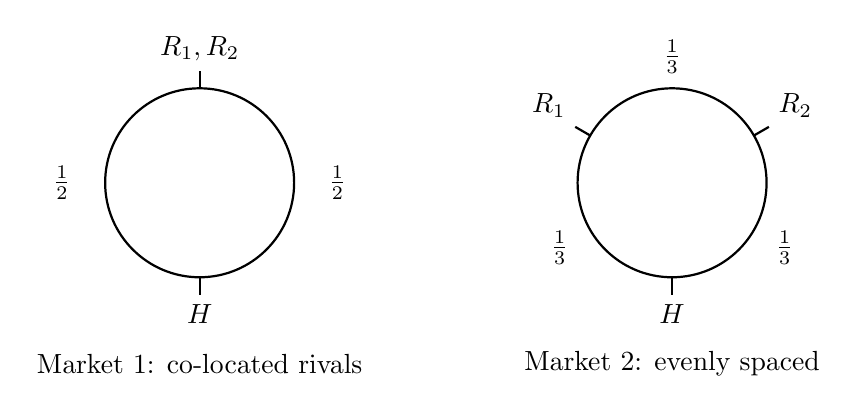
\begin{tikzpicture}[scale=1.0]
  \begin{scope}
    \draw[thick] (0,0) circle (1.2);
    \foreach \a/\lab/\pos in {90/{$R_1,R_2$}/above, 270/{$H$}/below}{
      \draw[thick] (\a:1.2) -- (\a:1.42);
      \node[\pos] at (\a:1.42) {\lab};
    }
    \node at (-1.75,0) {$\frac{1}{2}$};
    \node at (1.75,0) {$\frac{1}{2}$};
    \node at (0,-2.3) {Market 1: co-located rivals};
  \end{scope}
  \begin{scope}[xshift=6cm]
    \draw[thick] (0,0) circle (1.2);
    \foreach \a/\lab/\pos in {150/{$R_1$}/above left, 30/{$R_2$}/above right, 270/{$H$}/below}{
      \draw[thick] (\a:1.2) -- (\a:1.42);
      \node[\pos] at (\a:1.42) {\lab};
    }
    \node at (90:1.6) {$\frac{1}{3}$};
    \node at (210:1.65) {$\frac{1}{3}$};
    \node at (330:1.65) {$\frac{1}{3}$};
    \node at (0,-2.3) {Market 2: evenly spaced};
  \end{scope}
\end{tikzpicture}
\caption{The two hypothetical markets of the theory. Each circle has circumference one, and the fractions give the
arc lengths between neighboring hospitals. In market 1 the rivals $R_1$ and $R_2$ are co-located opposite $H$. In
market 2 the three hospitals are evenly spaced. Redrawn from \citet{Dafny2005}, Figure 1.}
\label{fig:11-dafny}
\end{figure}

Consider market 1 before the rivals merge. Co-located rivals are undifferentiated Bertrand competitors, so they
price at cost, $p_{R}=0$. A consumer at distance $x$ from $H$ is at distance $\frac{1}{2}-x$ from the rivals. She
buys from $H$ if $p_H+tx\le t(\frac{1}{2}-x)$, that is if $x\le\frac{1}{4}-\frac{p_H}{2t}$. Counting both sides of
$H$, its profit is
\begin{equation*}
\pi_H=p_H\cdot2\Big(\frac{1}{4}-\frac{p_H}{2t}\Big).
\end{equation*}
The first-order condition $\frac{1}{2}-\frac{2p_H}{t}=0$ gives $p_H^*=\frac{t}{4}$. Now let the rivals merge into
one firm $R$ with price $p_R$. The indifferent consumer moves to $x=\frac{1}{4}-\frac{p_H-p_R}{2t}$, and
\begin{equation*}
\pi_H=p_H\cdot2\Big(\frac{1}{4}-\frac{p_H}{2t}+\frac{p_R}{2t}\Big).
\end{equation*}
The first-order condition is $\frac{1}{2}-\frac{2p_H}{t}+\frac{p_R}{t}=0$. By symmetry $p_H=p_R$, so
$p_H^*=\frac{t}{2}$. The merger of co-located rivals doubles $H$'s price. Before the merger the rivals priced at
cost. After it they price like a differentiated firm, and $H$ responds to their higher price.

In market 2 the three hospitals are $\frac{1}{3}$ apart. Before the merger the standard symmetric Salop
equilibrium gives $p_H^*=\frac{t}{3}$. Suppose that after the merger one rival facility closes and the other stays
put, so $H$ and $R$ are $\frac{1}{3}$ apart on one side and $\frac{2}{3}$ on the other. $H$'s demand is
$\frac{1}{6}+\frac{p_R-p_H}{2t}$ on the short arc plus $\frac{1}{3}+\frac{p_R-p_H}{2t}$ on the long arc. Profit
$p_H(\frac{1}{2}+\frac{p_R-p_H}{t})$ gives the condition $\frac{1}{2}+\frac{p_R}{t}-\frac{2p_H}{t}=0$, so
$p_H^*=\frac{t}{2}$ at the symmetric equilibrium. The increase is from $\frac{t}{3}$ to $\frac{t}{2}$, or 50\%,
against 100\% in market 1. Mergers of co-located rivals raise prices more because the merger removes a fiercer
pre-merger rivalry.

These formulas hold when $t$ is small relative to $v$, so that every consumer buys and the hospitals compete for
the marginal consumer. Market 1 requires $t<\frac{4v}{3}$ after the merger and market 2 requires
$t<\frac{6v}{5}$. For larger $t$ the marginal consumer's reservation value binds, and demand has a kink. Dafny's
Appendix 1 gives the full solutions:
\begin{align*}
\text{Market 1:}\quad
p_H^{*,pre}&=\begin{cases}\frac{t}{4}, & t<\frac{8v}{3},\\[2pt] 2v-\frac{t}{2}, & \frac{8v}{3}<t<3v,\\[2pt] \frac{v}{2}, & t>3v,\end{cases}
&
p_H^{*,post}&=\begin{cases}\frac{t}{2}, & t<\frac{4v}{3},\\[2pt] v-\frac{t}{4}, & \frac{4v}{3}<t<2v,\\[2pt] \frac{v}{2}, & t>2v,\end{cases}\\[4pt]
\text{Market 2:}\quad
p_H^{*,pre}&=\begin{cases}\frac{t}{3}, & t<2v,\\[2pt] v-\frac{t}{6}, & 2v<t<3v,\\[2pt] \frac{v}{2}, & t>3v,\end{cases}
&
p_H^{*,post}&=\begin{cases}\frac{t}{2}, & t<\frac{6v}{5},\\[2pt] v-\frac{t}{3}, & \frac{6v}{5}<t<\frac{3v}{2}.\end{cases}
\end{align*}
In the middle ranges the hospitals price so that the consumer midway between them gets zero surplus. Take market 1
before the merger. Consumers within $\frac{v}{t}$ of the rivals buy from them at price zero. $H$ can sell to
everyone else only if the consumer at distance $\frac{1}{2}-\frac{v}{t}$ from $H$ gets zero surplus from $H$. That
condition gives $p_H=v-t(\frac{1}{2}-\frac{v}{t})=2v-\frac{t}{2}$.\footnote{For market 2 after the merger, the
appendix gives $\frac{v}{2}$ for all $t>\frac{3v}{2}$. Our derivation differs on part of this range. For
$\frac{3v}{2}<t<3v$ the two remaining hospitals are local monopolists on the long arc but still compete on the
short arc. Their symmetric equilibrium price is $\frac{2v}{5}+\frac{t}{15}$ for $\frac{3v}{2}<t<\frac{18v}{7}$ and
$v-\frac{t}{6}$ for $\frac{18v}{7}<t<3v$, and it is $\frac{v}{2}$ only for $t>3v$. We checked numerically that these
prices are equilibria and that $\frac{v}{2}$ is not. The difference lies outside
the range used for the comparison in the text.} \Cref{fig:11-dafny-prices} plots the solutions with $v=1$.

\begin{figure}[htbp]
\centering
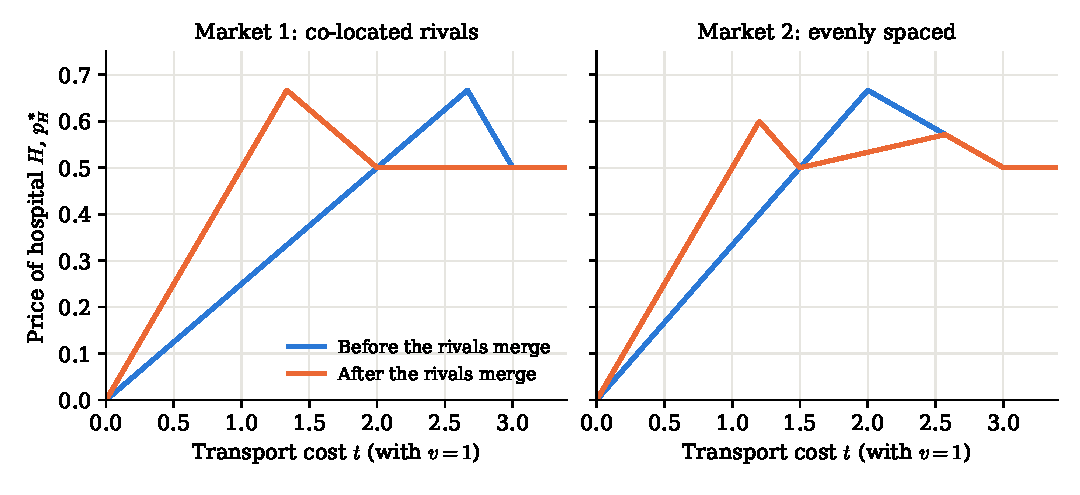
\includegraphics[width=0.95\textwidth]{figures/ch11/dafny_salop_prices.pdf}
\caption{Equilibrium price of hospital $H$ before and after its two rivals merge, as a function of the transport
cost $t$, with $v=1$. Left: co-located rivals. Right: evenly spaced hospitals, one of whose rival facilities closes
after the merger. Solutions from \citet{Dafny2005}, Appendix 1, with the market-2 post-merger curve for
$t>\frac{3}{2}$ derived in the footnote.}
\label{fig:11-dafny-prices}
\end{figure}

Dafny reports that with $v=1$ the average price increase is 66.7\% in market 1 and 40\% in market 2 (footnote 37).
We can reproduce these numbers as percentage gaps between average post-merger and average pre-merger prices. The
averages are taken over the range of $t$ in which the post-merger hospitals still compete, $t<2v$ in market 1 and
$t<\frac{3v}{2}$ in market 2. In
market 1 the average pre-merger price over $(0,2)$ is $0.250$ and the average post-merger price is $0.417$. In market
2 the averages over $(0,\frac{3}{2})$ are $0.250$ and $0.350$. Two predictions follow. Co-located hospitals are more
likely to merge, because they gain more market power and can cut duplicate departments. And a merger of
co-located rivals raises the prices of nearby hospitals by more. The number of co-located rival pairs near a
hospital is therefore a candidate instrument for exposure to rival mergers.

\casehead{Setting} Until 1984 hospitals were paid largely on a cost-plus basis. Medicare's Prospective Payment
System of 1984 paid a fixed amount per admission in each diagnosis-related group, and by 1989 most hospitals lost
money on Medicare patients. Managed care rose from under 30\% of private insurance in 1988 to nearly 95\% by 1999,
replacing fee-for-service payment with negotiated prices. There were 190 hospital mergers between 1989 and 1996,
against 74 between 1983 and 1988. Since 1991 the agencies had tried to block seven hospital mergers and lost every
time, often because courts accepted that non-profit hospitals would not exploit market power (printed pp.~8--9).

\casehead{Data} Merger data come from \citet{DranoveLindrooth2003}, who identify 97 independent hospital mergers
between 1989 and 1996. An independent merger combines two hospitals outside any system into a single entity that
reports one set of accounts and surrenders a license. The sample starts from general, non-federal hospitals in the
1988 American Hospital Association survey, located in metropolitan areas or counties with more than 100,000
residents. Price comes from Medicare cost reports. It is non-Medicare inpatient revenue per case-mix-adjusted
non-Medicare discharge, with charges deflated by each hospital's contractual discounts and Medicare's case-mix
index as a proxy for the non-Medicare one. The tails at the 5th and 95th percentiles are censored. Co-location is
measured from geocoded addresses. Two hospitals are co-located if they are within 0.3 miles as the crow flies and
no more than five blocks apart. Of 213 hospitals within 0.3 miles of another, 191 (3.6\% of 5,373) pass the map
check (printed pp.~12--15).

\Cref{tab:11-dafny-data} summarizes the two samples. In the All Hospitals sample of 4,487 hospitals, 178 (4.0\%)
merged and 163 (3.6\%) were co-located. Eighteen of the 163 merged, a rate of 11\% against 3.7\% for other hospitals.
The Rivals Sample contains the 877 non-merging hospitals with at least two rivals within 7 miles and complete price
data. Of these, 118 had a merging rival (NMW, for non-merging with merging rivals) and 759 did not (NMWO). The two
groups differ. NMW hospitals have nearly twice as many rivals, more Medicaid patients and slightly higher penetration of health maintenance organizations (HMOs).
Their prices grew by $-2.9\%$ between 1985 and 1988, against $4.2\%$ for NMWO hospitals. Treating rival mergers as
exogenous would therefore understate their effect.

\begin{table}[htbp]
\centering
\caption{Hospital mergers: sample means}
\label{tab:11-dafny-data}
\footnotesize
\begin{tabular}{@{}lcccc@{}}
\toprule
& All hospitals & \multicolumn{3}{c}{Rivals Sample} \\
\cmidrule(l){3-5}
& & All & NMW & NMWO \\
\midrule
1988 price (\$ of 2000) & 3,404 & 4,057 & 3,737 & 4,107 \\
1997 price (\$ of 2000) & 3,851 & 4,091 & 3,823 & 4,133 \\
$\ln p_{1988}-\ln p_{1985}$ & 0.064 & 0.032 & $-0.029$ & 0.042 \\
$\ln p_{1997}-\ln p_{1988}$ & 0.132 & 0.010 & 0.020 & 0.009 \\
$\ln p_{2000}-\ln p_{1997}$ & 0.013 & 0.001 & 0.039 & $-0.005$ \\
Merged, 1989--1996 (\%) & 4.0 & & & \\
Co-located (\%) & 3.6 & & & \\
Number of rival mergers, $R_i$ & & 0.156 & 1.161 & 0 \\
Number of co-located rival pairs, $Z_i$ & & 0.332 & 0.712 & 0.273 \\
Number of rivals within 7 miles & 3.16 & 7.37 & 12.03 & 6.64 \\
Medicaid share of discharges (\%) & 11.4 & 11.2 & 15.1 & 10.6 \\
County HMO penetration (\%) & 14.5 & 21.3 & 23.7 & 20.9 \\
Hospitals & 4,487 & 877 & 118 & 759 \\
\bottomrule
\end{tabular}

\smallskip
\begin{minipage}{0.9\linewidth}
\footnotesize Notes: NMW (NMWO) are non-merging hospitals with (without) a rival within 7 miles that merged in
1989--1996. Price change variables are censored at the 5th and 95th percentiles. Characteristics are for 1988,
HMO penetration for 1994. Selected rows. Source: \citet{Dafny2005}, Table 1.
\end{minipage}
\end{table}

\casehead{Estimating equations} For hospital $i$ in the Rivals Sample, let $R_i$ be the number of rival mergers
within 7 miles between 1989 and 1996. Let $Z_i$ be the number of co-located rival pairs within 7 miles in 1988,
excluding any pair to which $i$ belongs. Let $X_i$ be a vector of 1988 hospital and market characteristics. The outcome is
the change in log price between 1988 and 1997, $\Delta\ln p_i$, which spans the year before the first merger to the
year after the last. Because the instrument predicts whether but not when a rival merges, the design uses one
long difference. The equations are
\begin{align}
\text{first stage:}\qquad & R_i=\pi Z_i+X_i^{\top}\omega_F+u_i,\label{eq:11-dafny-fs}\\
\text{reduced form:}\qquad & \Delta\ln p_i=\phi Z_i+X_i^{\top}\omega_R+\varepsilon^{R}_i,\label{eq:11-dafny-rf}\\
\text{structural equation:}\qquad & \Delta\ln p_i=\beta R_i+X_i^{\top}\omega+v_i.\label{eq:11-dafny-iv}
\end{align}
Here $\varepsilon^R_i$ is an error term.\footnote{Here $\varepsilon^R_i$ denotes a regression error, not an
elasticity.} The coefficient $\beta$ is the effect of one rival merger on a hospital's price growth. OLS on
\eqref{eq:11-dafny-iv} is biased if $\Cov(R_i,v_i)\neq0$. The NMW and NMWO comparison above suggests that markets
with mergers had weaker price growth for other reasons, which biases OLS downward.

\casehead{The IV estimator} With one endogenous regressor and one instrument, the model is exactly identified. Let
$\tilde Z_i$ be the residual from regressing $Z_i$ on $X_i$. By the Frisch-Waugh-Lovell theorem, the OLS
coefficients on $Z_i$ in \eqref{eq:11-dafny-fs} and \eqref{eq:11-dafny-rf} are
$\hat\pi=\frac{\sum_i\tilde Z_iR_i}{\sum_i\tilde Z_i^2}$ and
$\hat\phi=\frac{\sum_i\tilde Z_i\Delta\ln p_i}{\sum_i\tilde Z_i^2}$. The IV estimator of $\beta$ is
\begin{equation}\label{eq:11-wald}
\hat\beta_{IV}=\frac{\sum_i\tilde Z_i\,\Delta\ln p_i}{\sum_i\tilde Z_i\,R_i}=\frac{\hat\phi}{\hat\pi},
\end{equation}
the ratio of the reduced-form coefficient to the first-stage coefficient. Substituting \eqref{eq:11-dafny-iv} shows
$\hat\beta_{IV}=\beta+\frac{\sum_i\tilde Z_iv_i}{\sum_i\tilde Z_iR_i}$, which converges to $\beta$ under two
conditions (\cref{app:econometrics}). \emph{Relevance} requires $\pi\neq0$. \emph{Exclusion} requires
$\E[\tilde Z_iv_i]=0$. Co-location of rivals must affect price growth only through the mergers it induces. Suppose the
effect of a rival merger differs across hospitals and co-location never makes a merger less likely. IV then
estimates a weighted average of the effects of the mergers that co-location induces \citep{ImbensAngrist1994}.

Dafny defends exclusion on three grounds. Location is nearly fixed. There has been very little hospital entry since
the Hill-Burton Act of 1946, so co-location in 1988 cannot reflect entry in anticipation of price growth during
1988--1996. Fewer than 1\% of sample hospitals had a rival that exited, and controlling for exits leaves the results
unchanged (footnote 27). The theory is then used to sign the most likely omitted factor, the growth of managed
care. Managed care lowered buyers' willingness to pay, which acts like a fall in $v$. In the solutions above, $v$
matters only in the kinked ranges, where the pre-merger price falls two for one with $v$ in market 1 and one for one
in market 2. Dafny argues that over the relevant range of $t$, prices are at least as sensitive to $v$ where rivals
are co-located. The spread of managed care should then, if anything, slow price growth in those markets and bias
the estimate toward zero (printed p.~22). Finally, the exclusion restriction has testable implications, discussed
next.

\casehead{Results} \Cref{tab:11-dafny} collects the main estimates. Co-location raises a hospital's own probability
of merging by 6.6 percentage points (6.2 with state fixed effects). In the Rivals Sample one more co-located rival
pair raises the number of rival mergers by 0.119 (0.112 with state fixed effects), against a mean of 0.16. The
implied first-stage $F$ statistic is about $(\frac{0.119}{0.018})^2\approx44$, so the instrument is strong. The
reduced form for 1988--1997 is 0.045, against mean price growth of 0.010. The IV estimate is the ratio
\eqref{eq:11-wald}:
\begin{equation*}
\hat\beta_{IV}=\frac{\hat\phi}{\hat\pi}=\frac{0.045}{0.119}\approx0.376,\qquad e^{0.376}-1\approx46\%.
\end{equation*}
The ratio of the rounded coefficients is 0.378. The paper reports 0.376, which equals the ratio of the unrounded
coefficients (footnote 29). With state fixed effects the estimate is 0.301, or about 35\%. A rival merger thus raised
nearby hospitals' prices by about 40\%, enough to move a hospital from the 25th to the 65th percentile of price
growth. OLS gives 0.016 and $-0.003$, both insignificant, and a Hausman test rejects their equality with the IV
estimates.

\begin{table}[htbp]
\centering
\caption{Hospital mergers: first stage, reduced forms and the effect of rival mergers}
\label{tab:11-dafny}
\footnotesize
\begin{tabular}{@{}llccc@{}}
\toprule
Equation & Dependent variable & Without state FE & With state FE & $N$ \\
\midrule
\multicolumn{5}{@{}l}{\textit{A. First stage: coefficient on co-location}} \\
Own merger on own co-location & Merged, 1989--1996 & 0.066 (0.016) & 0.062 (0.016) & 4,487 \\
Rival mergers on $Z_i$, \eqref{eq:11-dafny-fs} & $R_i$ & 0.119 (0.018) & 0.112 (0.019) & 877 \\
\addlinespace
\multicolumn{5}{@{}l}{\textit{B. Reduced form: coefficient on $Z_i$, \eqref{eq:11-dafny-rf}}} \\
Placebo, before the wave & $\ln p_{1988}-\ln p_{1985}$ & $-0.016$ (0.010) & $-0.013$ (0.011) & 877 \\
Treatment period & $\ln p_{1997}-\ln p_{1988}$ & 0.045 (0.014) & 0.034 (0.015) & 877 \\
Placebo, after the wave & $\ln p_{2000}-\ln p_{1997}$ & $-0.008$ (0.013) & $-0.001$ (0.014) & 703 \\
\addlinespace
\multicolumn{5}{@{}l}{\textit{C. Effect of rival mergers on $\ln p_{1997}-\ln p_{1988}$, \eqref{eq:11-dafny-iv}}} \\
IV, instrument $Z_i$ & & 0.376 (0.132) & 0.301 (0.147) & 877 \\
OLS & & 0.016 (0.026) & $-0.003$ (0.027) & 877 \\
\bottomrule
\end{tabular}

\smallskip
\begin{minipage}{0.97\linewidth}
\footnotesize Notes: Standard errors in parentheses. All specifications include the hospital characteristics
(ownership, teaching status, Medicaid share, debt-to-asset ratio, occupancy, bed-size categories) and market
characteristics (metropolitan-area population categories, HMO penetration, log per-capita income). Panel A, first row: All
Hospitals sample, linear probability model. Other rows: Rivals Sample. Source: \citet{Dafny2005}, Tables 2, 3 and
4.
\end{minipage}
\end{table}

\casehead{Tests of the exclusion restriction} The reduced forms in Panel B are falsification tests. Co-located rival
pairs predict price growth only during the merger wave. Before it (1985--1988) the coefficient is small and
negative, and after it (1997--2000) it is close to zero. The mergers thus appear to have caused a one-time increase
in price levels, with no lasting change in trend. The pre-period test matters because NMW hospitals had lower
pre-period growth in the raw data. An overidentification test uses two instruments, the numbers of rival pairs less
than 0.2 miles apart and 0.2 to 0.3 miles apart. The statistic $N R^2$ from regressing the 2SLS residuals on all
exogenous variables is 0.36, with a $p$-value of 0.55 under a $\chi^2(1)$ distribution \citep{Hausman1983}. Such a
test has power only against violations that differ between the two distance bands.

\casehead{Robustness} \Cref{tab:11-dafny-rob} reports the main sensitivity checks. Across co-location definitions
the 7-mile estimates range from 0.326 to 0.511. The market radius matters more. With a 5-mile radius the estimates
more than double, and with 10 miles they are small and insignificant. Effects concentrated on the closest rivals are
what the spatial model predicts, and they suggest that hospital markets are smaller than the 15 to 20 miles often
assumed. Dropping all controls barely changes the estimate (0.352 against 0.380 in the baseline of the appendix
table). By the logic of \citet{AltonjiElderTaber2005}, this stability suggests that unobserved characteristics,
if they relate to the instrument as the observed ones do, do not drive the result. Controlling for the number of
rivals, dropping co-located hospitals, using a negative binomial first stage, or using price levels gives estimates
of the same sign and similar size.

\begin{table}[htbp]
\centering
\caption{Hospital mergers: sensitivity of the IV estimate}
\label{tab:11-dafny-rob}
\footnotesize
\begin{tabular}{@{}lcccc@{}}
\toprule
\multicolumn{5}{@{}l}{\textit{A. Market radius and co-location definition}} \\
& 0.2 miles & 0.3 miles & 0.3 miles and $\le5$ blocks & 0.4 miles \\
\midrule
5 miles ($N=722$) & 0.992 (0.687) & 0.851 (0.340) & 0.962 (0.377) & 1.116 (0.603) \\
7 miles ($N=877$) & 0.511 (0.298) & 0.326 (0.125) & 0.376 (0.132) & 0.431 (0.221) \\
10 miles ($N=1{,}041$) & 0.046 (0.082) & 0.038 (0.050) & 0.051 (0.054) & 0.021 (0.072) \\
\bottomrule
\end{tabular}

\bigskip
\begin{tabular}{@{}lcc@{}}
\toprule
\multicolumn{3}{@{}l}{\textit{B. Specification checks (7 miles, 0.3 miles and $\le5$ blocks)}} \\
Specification & Estimate & $N$ \\
\midrule
(1) Baseline & 0.380 (0.132) & 877 \\
(2) No hospital or market controls & 0.352 (0.132) & 877 \\
(3) Dependent variable not censored & 0.402 (0.143) & 877 \\
(4) Dummies for the number of rivals & 0.408 (0.198) & 877 \\
(5) Co-located hospitals dropped & 0.326 (0.122) & 816 \\
(6) Negative binomial first stage & 0.222 (0.099) & 877 \\
(7) Change in price level (\$ of 2000) & 1,566 (563) & 877 \\
\bottomrule
\end{tabular}

\smallskip
\begin{minipage}{0.9\linewidth}
\footnotesize Notes: 2SLS estimates of $\beta$ in \eqref{eq:11-dafny-iv} without state fixed effects, standard
errors in parentheses. Panel A, column 3, row 2 is the main specification of \cref{tab:11-dafny}. Panel B, row 1
is printed as 0.380 in the appendix table and as 0.376 in the main table. Source: \citet{Dafny2005}, Table 5 and
Appendix Table 1.
\end{minipage}
\end{table}

\casehead{Interpretation} The estimates imply large price increases by the rivals of merging hospitals, about 40\%
per rival merger. Prior longitudinal studies, which compared merging and non-merging hospitals or treated rival
mergers as exogenous, found no effect or a negative one \citep{ConnorFeldman1998}. The OLS estimates here reproduce
that null, and the IV estimates show it to be a selection artifact. The magnitudes are close to those of
structural models of hospital choice, which predict increases of 10\% to 58\% for hypothetical mergers in markets
with few competitors \citep{CappsDranoveSatterthwaite2003,GaynorVogt2003}. Those predictions ignore rivals'
responses and may be too low for that reason (footnote 35). The retrospective thus supports prospective structural
analysis of hospital mergers. Combined with the 14\% cost reductions that \citet{DranoveLindrooth2003} find for the
same type of merger, the results imply large profit gains for merging hospitals.

\casehead{Limitations} The estimate is local. It measures the effect of the rival mergers that co-location induces,
which are mergers of undifferentiated hospitals with unusually large gains in market power. It measures rivals'
responses and says nothing direct about the merging hospitals' own prices, which may rise more or less. The
specification is linear in the number of rival mergers and ignores distance within the 7-mile circle. The price
measure relies on list charges, a contractual discount factor and the Medicare case-mix index. Prices are
negotiated with insurers, so the outcome reflects bargaining between hospitals and managed-care plans, which the
Salop model abstracts from \citep{GalOr1999,CappsDranoveSatterthwaite2003,Ho2009}. \citet{GowrisankaranNevoTown2015}
build this bargaining into a merger simulation for hospitals. They combine the simulation method of
\cref{sec:11-simulation} with the Nash-in-Nash bargaining framework of \citet{CrawfordYurukoglu2012}. They find
that insurers' bargaining power can substantially counteract the market power that hospital mergers create
\citep[p.~238]{AskerNocke2021}. The exclusion restriction can
fail if co-located hospitals sit in old urban cores whose demand evolved differently during the 1990s. The placebo
regressions address this concern only for the years around the wave. Finally, the long difference uses only
cross-sectional variation, so the timing of mergers is not exploited.

\casehead{Contribution} The paper shows how to combine rival analysis with an instrument, so that a retrospective
can address the selection of mergers. It produced the first observational evidence of large price effects of
hospital mergers and showed that relevant hospital markets are small. It also lent support to the structural models
used to evaluate proposed hospital mergers. The idea transfers to other industries in which distance in physical or
product space shifts the propensity to merge.

\subsection{What the retrospective literature finds}\label{sec:11-retro-lit}

The three studies above are part of a growing literature. \citet[Section 3.7 and Appendix A]{AskerNocke2021} survey
the retrospectives published between 2000 and 2020 in the leading general-interest journals and the main industrial
organization journals. For each study they record the date of the transaction, the country and the industry, and
they quote the sentence that best states the authors' conclusion. They chose quotes over a standardized measure of
the price effect, because studies differ too much in units, outcomes and focus (p.~256, n.~201).

Three selection issues limit what the collection can teach \citep[pp.~255--256]{AskerNocke2021}. First, the studied
mergers were cleared by the authorities, so blocked and deterred mergers are absent (\cref{sec:11-retro-select}).
Second, the studies come from industries where data are available, which tilts the sample toward consumer-facing
markets and regulated industries with administrative data. Few retrospectives study intermediate goods. Third, the
studied mergers tend to be large or to offer a chance to study some phenomenon of interest. The collection is not a
random sample of cleared mergers.

Five themes emerge \citep[p.~257]{AskerNocke2021}.
\begin{enumerate}[label=(\roman*)]
\item The price effects vary widely. Some prices rise, at times by a lot, others do not move, and some fall. Asker
and Nocke find this range the most striking feature of the literature.
\item Few studies estimate the change in consumer welfare. Many treat price changes as a sufficient statistic.
\item The outcome variables differ. Most studies measure the prices of the merging firms' products. Some also measure
rivals' prices, and others measure quantities or market shares.
\item Few studies examine longer-run dynamics. \citet{FocarelliPanetta2003} compare short-run and long-run price
effects, and \citet{IgamiUetake2019} study innovation.
\item Few retrospectives study product quality, variety, entry and exit, or investment.
\end{enumerate}
\Cref{tab:11-retro-lit} reproduces a selection of the entries, chosen to cover the range of industries and findings.
Read together, the studies show that consummated mergers can harm consumers, which supports the value of merger
review. The range of outcomes also argues for evaluating each merger in the context of its industry
\citep[p.~257]{AskerNocke2021}.

\begin{table}[htbp]
\centering
\caption{A selection of merger retrospectives}
\label{tab:11-retro-lit}
\footnotesize
\setlength{\tabcolsep}{3pt}
\begin{tabularx}{\textwidth}{@{}>{\raggedright\arraybackslash}p{1.45cm}>{\raggedright\arraybackslash}p{1.16cm}%
>{\raggedright\arraybackslash}p{1.91cm}>{\raggedright\arraybackslash}X>{\raggedright\arraybackslash}p{2.15cm}@{}}
\toprule
Date & Country & Industry & Main finding & Study \\
\midrule
\multicolumn{5}{@{}l}{\textit{Single transactions}} \\
1987 & USA & Airlines & Prices rose 5.0 to 6.0 percent on routes that one carrier served and the other could enter,
more than half the rise on routes where the two had competed &
\citet{KwokaShumilkina2010} \\
1997 & USA & Tampons, pads & Always pads up 8 percent and Tampax up 5 percent relative to private label &
\citet{Weinberg2011} \\
1999 & France & Supermarkets & Rivals' affected stores up about 2 percent (1.8 to 2.4), and the merging firms' prices up
4 to 5 percent & \citet{AllainEtAl2017} \\
1999 & USA & Gasoline & No evidence of higher prices & \citet{SimpsonTaylor2008} \\
2001 & Sweden & Beer & Merging firms' prices roughly constant around the merger, other main brewers' prices up
somewhat, divested beers down relative to both & \citet{FribergRomahn2015} \\
2006 & USA & Appliances & Increases for dishwashers and larger ones for dryers, none for refrigerators or washers.
The merged firm's share and product count fell & \citet{AshenfelterHoskenWeinberg2013} \\
2008 & USA & Airlines & Small fare effects where Delta and Northwest competed: insignificant in nonstop markets, 2.3
percent in connecting markets & \citet{Luo2014} \\
\addlinespace
\multicolumn{5}{@{}l}{\textit{Multiple transactions}} \\
1989--1996 & USA & Hospitals & Prices up roughly 40 percent after nearby rivals merge & \citet{Dafny2009} \\
1990--1998 & Italy & Retail banking & Adverse price changes are temporary, and in the long run efficiency gains dominate
& \citet{FocarelliPanetta2003} \\
1993--2000 & Canada & Mortgages & Significant average rise in interest rates, some borrowers unaffected, and lower price
dispersion & \citet{AllenClarkHoude2014} \\
1996--2006 & USA & Radio & Ad quantity down 11 percent and ad prices up 6 percent. Listener welfare up 0.2 percent,
advertiser welfare down 21 percent & \citet{Jeziorski2014} \\
1996--2015 & Global & Hard disk drives & The rule that blocks mergers when three or fewer firms exist is reasonably
close to maximizing discounted welfare & \citet{IgamiUetake2019} \\
1997--2010 & USA & Dialysis & In more than 1,200 acquisitions, acquired facilities raised doses of highly reimbursed
drugs, replaced skilled nurses with technicians and waitlisted fewer patients. Hospitalizations and mortality rose &
\citet{EliasonEtAl2020} \\
1997--2012 & USA & Hospitals & Of 28 mergers, 9 raised prices and 6 lowered them significantly relative to
controls. Mean change 8.9 percent, median 9.6 percent & \citet{Garmon2017} \\
1998--2000 & USA & Consumer goods & Four of five mergers raised some prices, typically by 3 to 7 percent &
\citet{AshenfelterHosken2010} \\
1998--2006 & USA & Health insurance & Premiums about 7 percentage points higher by 2007 from rising local
concentration, and monopsony power over physicians & \citet{DafnyDugganRamanarayanan2012} \\
2007--2011 & USA & Hospitals & Of 366 mergers, prices up more than 6 percent when the hospitals were within about 5
miles, no effect beyond about 25 miles & \citet{CooperEtAl2019} \\
2007--2008 & USA & Grocery & Five mergers raised prices by more than 2 percent (four in highly concentrated
markets), five lowered them by more than 2 percent, four had little effect & \citet{HoskenOlsonSmith2018} \\
\bottomrule
\end{tabularx}

\vspace{3pt}
\begin{minipage}{\textwidth}
\footnotesize Notes: Paraphrased from the quotations collected by \citet[Appendix A, pp.~262--265]{AskerNocke2021},
whose table lists the date of the transaction, the country, the industry and a quotation from each paper. The
radio entry was also checked against the author's manuscript of \citet{Jeziorski2014}. The appliance, hospital
(1989--1996) and consumer-goods entries are studied in \cref{sec:11-ah,sec:11-maytag,sec:11-dafny}.
\end{minipage}
\end{table}

\section{Does merger simulation work? The Swedish analgesics merger}\label{sec:11-bv}

A merger simulation (\cref{sec:11-simulation}) makes a prediction that can be checked. If a simulated merger is
later consummated, a retrospective of the kind developed in \cref{sec:11-retro} measures its actual effects, and the
two can be compared. Such validation studies are rare, because they need a merger that was simulated or could be
simulated with pre-merger data, and post-merger data on the same market. \citet{BjornerstedtVerboven2016} carry out
one for a merger of painkiller producers in Sweden. They built the simulation for the Swedish Competition Authority
during its review, before the outcome was known. A few years later they compared its predictions with what
happened.\footnote{We use pp.~134, 137 and 147 of the published article, which contain its Figures 1 and 2 and its
Table 6, and its abstract. The institutional facts, the data, the estimating equations, the instruments and the
robustness checks come from the January 2013 working paper \citep{BjornerstedtVerboven2013}. The published version
adds random coefficients models and re-estimates the nested logit, so the working-paper numbers differ from those of
its Table 6.}

\subsection{Question and setting}\label{sec:11-bv-setting}

\casehead{Question} Do the merger simulations used by competition authorities predict the price effects of actual
mergers? And which modeling choices matter for the answer?

\casehead{Setting} The market is over-the-counter analgesics in Sweden. Products differ by active substance
(paracetamol, ibuprofen and acetylsalicylic acid, ASA, sold as aspirin), by administrative form (ordinary tablets
and effervescent, or fizzy, tablets), and by brand, pack size and dose. In 2008 paracetamol held 42.1 percent of
sales value, ibuprofen 29.0 percent and ASA 28.9 percent \citep[Table 1]{BjornerstedtVerboven2013}. Paracetamol and
ibuprofen are sold mainly as tablets, and ASA mainly as fizzy tablets.

GlaxoSmithKline (GSK) notified its acquisition of AstraZeneca Tika (AZT) on December 22, 2008. The Swedish
Competition Authority cleared it on April 3, 2009 \citep[p.~6]{BjornerstedtVerboven2013}. The two firms were the
only sellers of paracetamol \citep[p.~137]{BjornerstedtVerboven2016}. AZT sold Alvedon, with 29.3 percent of 2008
sales value, and Reliv, with 2.2 percent. GSK sold Panodil, with 10.6 percent. McNeil led the other two segments,
with Ipren in ibuprofen (19.1 percent) and Treo and Magnecyl in ASA (25.6 percent together). Nycomed, Meda and Bayer
held the remaining 13.2 percent \citep[Table 2]{BjornerstedtVerboven2013}.

Until 2009 all sales went through the state pharmacy monopoly, Apoteket AB. It added a fixed percentage markup to
the producers' wholesale prices and charged the same price in every pharmacy, so producers set retail prices
indirectly \citep[pp.~6 and~9]{BjornerstedtVerboven2013}. The authority cleared the merger on two grounds. It
judged that consumers choose brands more than substances. It also expected the deregulation of pharmacies, decided
for 2009, to bring entry and stronger buyers. Its decision cited the authors' simulation as showing no significant
price increase. The authors note that their simulations predicted an insignificant increase only in a scenario with
large efficiencies (pp.~6--8). Entry after the deregulation was surprisingly slow
\citep[p.~134]{BjornerstedtVerboven2016}. Ibuprofen and ASA are therefore the substitutes that discipline the
paracetamol price.

\casehead{Data} During its review the authority obtained monthly sales data for 1995 to 2008 from Apoteket. A
product is a brand, form, pack size and dose, such as Alvedon tablets in packs of 30 pieces of 500 mg. An
observation of product $j$ in month $t$ records the price $p_{jt}$, the volume $q_{jt}$ and the revenue
$r_{jt}=p_{jt}q_{jt}$. Prices include value-added tax and are the prices every consumer paid. The data are merged
with monthly marketing expenditures by brand and with monthly counts of sick men and sick women from Statistics
Sweden. The full sample has 11,185 product-months. The estimation sample keeps the three main substances and the
two main forms. It has 7,240 product-months, about 43 products per month, and covers about 90 percent of sales value
\citep[Section 2.3]{BjornerstedtVerboven2013}. Painkillers have no natural unit of consumption. The authors measure
volume in tablets, in defined daily doses and in normal single doses, and they report results for tablets.
\Cref{tab:11-bv-sum} reproduces the main summary statistics. For the retrospective the authors later obtained the
same data for 2008 to May 2011. The 2008 figures matched those of the original data (p.~10).

\begin{table}[htbp]
\centering
\caption{Swedish analgesics: summary statistics of the estimation sample, 1995--2008}
\label{tab:11-bv-sum}
\footnotesize
\begin{tabular}{@{}lcccc@{}}
\toprule
Variable & Mean & Std.\ dev. & Min. & Max. \\
\midrule
Revenue $r_{jt}$ (million SEK) & 1.24 & 2.56 & 0.00 & 22.95 \\
Price per tablet $p_{jt}$ (SEK) & 1.06 & 0.46 & 0.27 & 2.55 \\
Tablets sold $q_{jt}$ (million) & 1.11 & 2.19 & 0.00 & 16.61 \\
Marketing expenditures & 564.1 & 1{,}445.7 & 0 & 13{,}536 \\
Sick women & 822.9 & 197.0 & 391 & 1{,}204 \\
Sick men & 524.5 & 108.0 & 254 & 763 \\
Nominal GDP (billion SEK) & 621.6 & 107.4 & 443.2 & 859.7 \\
\bottomrule
\end{tabular}

\smallskip
\begin{minipage}{0.8\linewidth}
\footnotesize Notes: 7,240 product-months. Selected rows. The paper does not state the units of marketing
expenditures and of the sickness counts. In December 2008 one euro was 10.8 SEK and one US dollar 8.0 SEK. Source:
\citet{BjornerstedtVerboven2013}, Table 3.
\end{minipage}
\end{table}

\subsection{The retrospective evidence}\label{sec:11-bv-retro}

\Cref{fig:11-bvprice,fig:11-bvshare} show what happened. Paracetamol prices drifted up from about 1.39 kronor in
April 2007 to about 1.50 at the end of 2008. Within two months of the merger they jumped to about 1.99 and stayed
near that level. Ibuprofen prices, at about 1.67, did not move at the merger. ASA prices rose modestly, from about
1.41 to about 1.55 kronor. These readings are taken from the figure.
In logs the plotted paracetamol jump is about $\ln\frac{1.99}{1.50}\approx0.28$, and the ASA increase is about
$\ln\frac{1.55}{1.41}\approx0.10$. The paracetamol share of the analgesics market fell from a peak of about
49\% just before the merger to about 41\%, then recovered to 43\% to 45\%. The ibuprofen share jumped from about
27\% to about 32\%, and the ASA share stayed near 24\% to 26\%. Consumers substituted mainly toward ibuprofen.

\begin{figure}[htbp]
\centering
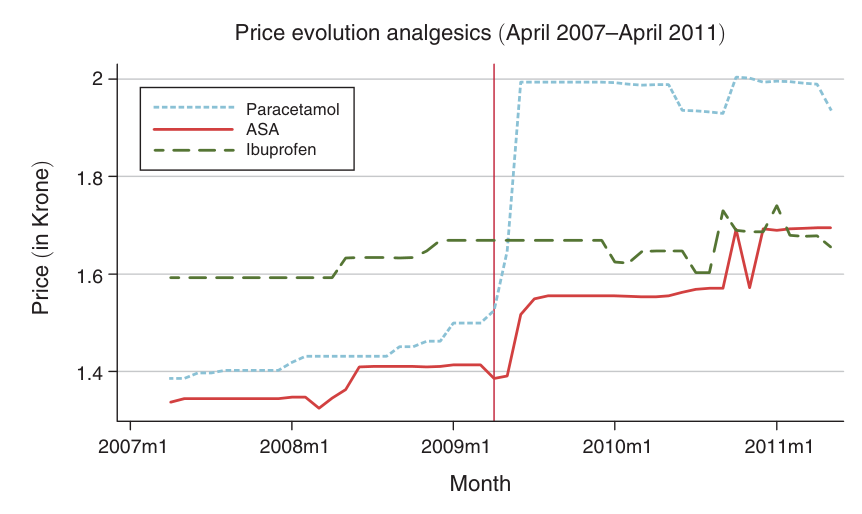
\includegraphics[width=0.72\textwidth]{figures/ch11/bv_fig1_price.png}
\caption{Average prices of paracetamol, ASA and ibuprofen analgesics in Sweden, April 2007 to April 2011, in kronor.
The vertical line marks the merger (April 2009). Source: \citet{BjornerstedtVerboven2016}, Figure 1.}
\label{fig:11-bvprice}
\end{figure}

\begin{figure}[htbp]
\centering
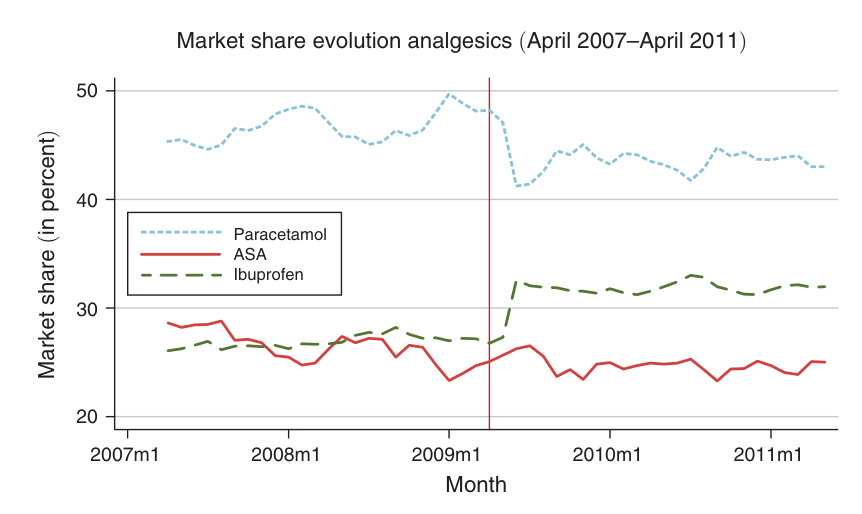
\includegraphics[width=0.72\textwidth]{figures/ch11/bv_fig2_share.png}
\caption{Market shares of paracetamol, ASA and ibuprofen analgesics in Sweden, April 2007 to April 2011, in percent.
The vertical line marks the merger (April 2009). Source: \citet{BjornerstedtVerboven2016}, Figure 2.}
\label{fig:11-bvshare}
\end{figure}

The stability of ibuprofen prices suggests that the paracetamol increase was not caused by a general cost or demand
shock \citep[p.~134]{BjornerstedtVerboven2016}. A regression in the spirit of \citet{AshenfelterHosken2010} makes
the comparison precise:
\begin{equation}\label{eq:11-bv-retro}
\ln p_{gt}=\alpha_g+\beta_g\,\mathit{PostMerger}_t+e_{gt}.
\end{equation}
Here $p_{gt}$ is the average price of product group $g$ in month $t$. The indicator $\mathit{PostMerger}_t$ equals
one after the merger. The published version defines groups by substance and by substance and firm (p.~134). Each group has its
own post-merger change $\beta_g$, which is more general than a common change for all control groups. The difference
between the merging firms' $\beta_g$ and a rival group's $\beta_g$ is a DiD estimate of the merger effect. By
\cref{prop:11-didbias}, a rival control yields a lower bound when rivals raise prices in response.

The published version compares one year before and one year after the merger. The short window keeps out later
effects of the deregulation \citep[p.~134 and eq.~(1)]{BjornerstedtVerboven2016}. The article reports that the
merging firms raised prices by 40 percent and that some outsiders raised prices by more than 10 percent
\citep[abstract]{BjornerstedtVerboven2016}. Its Table~4 gives price changes of 39.7 percent for paracetamol, 0.1
percent for ibuprofen and 13.3 percent for ASA (p.~135). \Cref{tab:11-bv-expost} reports the working paper's
estimates, in log points. They compare two years on each side of the
merger, April 2007 to April 2009 against May 2009 to May 2011, and define groups by substance and by firm
\citep[Table 7]{BjornerstedtVerboven2013}.

The paracetamol price rose by 0.351 log points, or 42 percent. Ibuprofen prices did not move (0.001), and ASA prices
rose by 0.100 log points, or 11 percent. With ibuprofen as the control the DiD estimate is 0.350. With ASA as the
control it is 0.251, or 29 percent. Pooling the two rival substances into one control gives 0.30, or 35 percent
\citep[fn.~17]{BjornerstedtVerboven2013}. The ASA increase is consistent with a rival response, so the ASA-based
estimate understates the effect on paracetamol prices. Both merging firms raised prices by similar amounts, 0.356 log
points for AZT and 0.379 for GSK. Among the outsiders, Bayer raised prices by 0.105 and McNeil by 0.084 log points.
The regressions compare average log prices of product groups over the two windows, so they need not match the jump
in the plotted average price.

The same design applied to volume shares shows where demand went. The paracetamol share fell by 3.3 percentage
points, with a 95 percent confidence interval of 2.7 to 3.9 points. The ibuprofen share rose by 5.0 points, and the
ASA share fell by 1.6 points. AZT lost 5.6 points, while GSK's loss of 0.3 points is insignificant. McNeil lost 2.7
points, and the other outsiders gained a little \citep[pp.~31--32]{BjornerstedtVerboven2013}.

\subsection{The prospective models}\label{sec:11-bv-model}

The simulation has the structure of \cref{sec:11-simulation}: estimate demand on pre-merger data, recover marginal
costs from the pre-merger first-order conditions, change the ownership matrix, and solve for the new equilibrium.
Two demand families are used, each in two versions.

\casehead{Nested logit} Consumer $i$ chooses among products $j\in\mathcal{J}$ and an outside good $j=0$. Products are
grouped into nests $g$, and each nest into subnests $h$. In the authors' maintained specification the nests are the
two administrative forms, and the subnests are the substances within each form
\citep[p.~20]{BjornerstedtVerboven2013}. We first present the one-level version, with nests $g$ only. Its utility is
\begin{equation*}
u_{ij}=\delta_j+\zeta_{ig}+(1-\sigma)\epsilon_{ij},
\end{equation*}
where $\delta_j$ is mean utility, $\epsilon_{ij}$ is type-I extreme value, and $\zeta_{ig}$ has the distribution
that makes $\zeta_{ig}+(1-\sigma)\epsilon_{ij}$ extreme value \citep{Cardell1997}. The nesting parameter
$\sigma\in[0,1)$ measures the correlation of tastes within a nest (\cref{ch:logit}). As in \cref{sec:11-diversion},
let $H_g=\sum_{k\in g}e^{\frac{\delta_k}{1-\sigma}}$. Market shares are
\begin{equation}\label{eq:11-nl-shares}
s_j=s_{j|g}\,s_g,\qquad s_{j|g}=\frac{e^{\frac{\delta_j}{1-\sigma}}}{H_g},\qquad s_g=\frac{H_g^{1-\sigma}}{1+\sum_{g'}H_{g'}^{1-\sigma}},
\end{equation}
and the outside share is $s_0=\frac{1}{1+\sum_{g'}H_{g'}^{1-\sigma}}$.

\begin{lemma}[Nested logit share derivatives]\label{lem:11-nl-deriv}
For products $j\neq k$,
\begin{align*}
\frac{\partial s_j}{\partial\delta_j}&=s_j\Big[\frac{1}{1-\sigma}-\frac{\sigma}{1-\sigma}s_{j|g}-s_j\Big],\\
\frac{\partial s_j}{\partial\delta_k}&=-s_j\Big[\frac{\sigma}{1-\sigma}s_{k|g}+s_k\Big]\quad\text{if $k$ is in $j$'s nest,}\\
\frac{\partial s_j}{\partial\delta_k}&=-s_js_k\quad\text{if $k$ is in another nest.}
\end{align*}
\end{lemma}

\begin{proof}
Taking logs of \eqref{eq:11-nl-shares} gives
$\ln s_j=\frac{\delta_j}{1-\sigma}-\sigma\ln H_g-\ln\big(1+\sum_{g'}H_{g'}^{1-\sigma}\big)$. \Cref{sec:11-diversion}
computed the derivatives of the last two terms on the way to \eqref{eq:11-nl-diversion}. The derivative of $\ln H_g$
with respect to $\delta_k$ is $\frac{s_{k|g}}{1-\sigma}$ for $k\in g$ and zero otherwise. The derivative of the log
of the denominator is $s_k$ for every inside product $k$. Hence $\frac{\partial\ln s_j}{\partial\delta_k}$ equals
$\frac{1}{1-\sigma}-\frac{\sigma}{1-\sigma}s_{j|g}-s_j$ for $k=j$, $-\frac{\sigma}{1-\sigma}s_{k|g}-s_k$ for $k\neq j$
in the same nest, and $-s_k$ for $k$ in another nest. Multiplying each by $s_j$ gives the lemma.
\end{proof}

Inverting \eqref{eq:11-nl-shares} gives the linear estimating equation
$\ln s_j-\ln s_0=\delta_j+\sigma\ln s_{j|g}$ (\cref{ch:logit}). The two-level version adds the subnests $h$ within
each nest $g$, with parameters $0\le\sigma_2\le\sigma_1<1$. Here $\sigma_1$ measures the correlation of tastes
within a subnest and $\sigma_2$ within a nest. With unit demand its estimating equation is
\begin{equation}\label{eq:11-nl2}
\ln s_j-\ln s_0=x_j\beta-\alpha\,p_j+\sigma_1\ln s_{j|hg}+\sigma_2\ln s_{h|g}+\xi_j,
\end{equation}
where $s_{j|hg}$ is $j$'s share of its subnest and $s_{h|g}$ the subnest's share of the nest
\citep[eq.~(9)]{Verboven1996,BjornerstedtVerboven2013}.\footnote{We verified \eqref{eq:11-nl2} and the derivatives
below numerically against the two-level share formulas.} The authors also estimated the reverse order, with
substances as nests and forms as subnests. It gave $\sigma_1<\sigma_2$, which is inconsistent with random utility
maximization, so they kept forms as the nests (p.~20). Let $\vartheta_1=\frac{1}{1-\sigma_1}-\frac{1}{1-\sigma_2}\ge0$,
$\vartheta_2=\frac{\sigma_2}{1-\sigma_2}$ and $s_{j|g}=s_{j|hg}s_{h|g}$. The share derivatives are
\begin{align*}
\frac{\partial s_j}{\partial\delta_j}&=s_j\Big[\frac{1}{1-\sigma_1}-\vartheta_1\,s_{j|hg}-\vartheta_2\,s_{j|g}-s_j\Big],\\
\frac{\partial s_j}{\partial\delta_k}&=-s_j\big[\vartheta_1\,s_{k|hg}+\vartheta_2\,s_{k|g}+s_k\big]\quad\text{(same subnest)},\\
\frac{\partial s_j}{\partial\delta_k}&=-s_j\big[\vartheta_2\,s_{k|g}+s_k\big]\quad\text{(same nest, other subnest)},\\
\frac{\partial s_j}{\partial\delta_k}&=-s_js_k\quad\text{(other nest)}.
\end{align*}
Cross-elasticities are largest within a subnest, smaller between subnests of the same nest, and smallest across
nests. Under the maintained order, the closest substitutes share both form and substance, and the most distant
differ in form. The estimates in \cref{tab:11-bv-demand} below show this ordering.

\casehead{Unit demand and constant expenditures} The two versions differ in how price enters utility and what a
market share measures \citep[Section 3.1]{BjornerstedtVerboven2013}. Consumer $i$, with income $y_i$, gets utility
$u_{ij}=x_j\beta+\xi_j+\alpha f(y_i,p_j)+\epsilon_{ij}$ from product $j$. Conditional on choosing $j$, she buys
$d_{ij}$ units, given by Roy's identity:
\begin{equation*}
d_{ij}=-\dfrac{\frac{\partial f(y_i,p_j)}{\partial p_j}}{\frac{\partial f(y_i,p_j)}{\partial y_i}} .
\end{equation*}
Unit demand sets $f(y_i,p_j)=y_i-p_j$. Both derivatives have absolute value one, so $d_{ij}=1$. Constant
expenditures sets $f(y_i,p_j)=\frac{1}{\gamma}\ln y_i-\ln p_j$ for a constant $\gamma\in(0,1)$. Then
\begin{equation*}
d_{ij}=-\dfrac{-\frac{1}{p_j}}{\frac{1}{\gamma y_i}}=\frac{\gamma y_i}{p_j},
\end{equation*}
so the consumer spends the fraction $\gamma$ of her income on the chosen product. In both versions the income term
is common to all products of consumer $i$, so it drops out of the choice probabilities. These remain the nested logit
formulas, now evaluated at the mean utilities given below. Summing $d_{ij}$ times the choice probability over
consumers gives aggregate demand. With unit demand $q_j=s_jM$, where $M$ is the number of consumers. With constant
expenditures $q_j=\frac{s_jB}{p_j}$, where $B=\gamma\sum_iy_i$ is the potential budget for the category.

In the \emph{unit demand} version each consumer buys at most one unit. Mean utility is linear in price,
$\delta_j=x_j\beta-\alpha p_j+\xi_j$, and shares are volume shares, $s_j=\frac{q_j}{M}$ for a potential number of
units $M$. Since $\frac{\partial\delta_k}{\partial p_k}=-\alpha$, the elasticities in the one-level model are
\begin{align}
\varepsilon_{jj}&=-\alpha\,p_j\Big[\frac{1}{1-\sigma}-\frac{\sigma}{1-\sigma}s_{j|g}-s_j\Big],\label{eq:11-unit-own}\\
\varepsilon_{jk}&=\alpha\,p_k\Big[\frac{\sigma}{1-\sigma}s_{k|g}+s_k\Big]\ \text{(same nest)},\qquad
\varepsilon_{jk}=\alpha\,p_ks_k\ \text{(other nest)},\nonumber
\end{align}
where $\varepsilon_{jj}<0$ is the own-price elasticity in signed form. Elasticities are proportional to price.
Expensive products have more elastic demand, and the own elasticity of a product rises as its price rises.

In the \emph{constant expenditures} version each consumer spends a fixed budget on the category. Mean utility is
linear in log price, $\delta_j=x_j\beta-\alpha\ln p_j+\xi_j$, and shares are value shares,
$w_j=\frac{p_jq_j}{B}$ for a potential budget $B$. The formulas \eqref{eq:11-nl-shares} now give $w_j$. Quantity is
$q_j=\frac{Bw_j}{p_j}$, so $\ln q_j=\ln B+\ln w_j-\ln p_j$, and $\frac{\partial\delta_k}{\partial\ln
p_k}=-\alpha$. The quantity elasticities are
\begin{align}
\varepsilon_{jj}&=-\alpha\Big[\frac{1}{1-\sigma}-\frac{\sigma}{1-\sigma}w_{j|g}-w_j\Big]-1,\label{eq:11-ce-own}\\
\varepsilon_{jk}&=\alpha\Big[\frac{\sigma}{1-\sigma}w_{k|g}+w_k\Big]\ \text{(same nest)},\qquad
\varepsilon_{jk}=\alpha\,w_k\ \text{(other nest)}.\nonumber
\end{align}
These depend on prices only through value shares, so they are roughly constant along the demand curve. The extra
$-1$ in the own elasticity reflects the fixed budget. A higher price lowers the quantity bought even at an unchanged
value share, and that lost quantity is diverted to no other product.

Substituting value shares into the inverted two-level system gives the constant-expenditure estimating equation
\begin{equation}\label{eq:11-ce-est}
\ln w_j-\ln w_0=x_j\beta-\alpha\ln p_j+\sigma_1\ln w_{j|hg}+\sigma_2\ln w_{h|g}+\xi_j,
\end{equation}
where $w_0=1-\sum_kw_k$ is the outside value share. Here $w_{j|hg}$ and $w_{h|g}$ are the value shares within the
subnest and the nest \citep[eq.~(10)]{BjornerstedtVerboven2013}. The equation differs from \eqref{eq:11-nl2} in three ways.
Price enters in logs, shares are measured in value, and the potential market is a budget $B$ rather than a number of
consumers. The authors note that this version had not been used in empirical work, although it is as easy to
estimate as the unit-demand version (pp.~2--3).

The difference matters for mergers through pass-through (\cref{sec:11-passthrough}). Under unit demand, demand becomes
more elastic as price rises, which restrains post-merger price increases. Under constant expenditures, the merged
firm faces roughly constant elasticities and can push prices further. The contrast is the one between linear or
logit demand and the constant-expenditure logit in \cref{fig:11-curvature}.

\casehead{Random coefficients} The nested logit restricts substitution to the hierarchy of nests and subnests. It
also rules out correlated preferences along continuously measured characteristics
\citep[p.~137]{BjornerstedtVerboven2016}. The published version therefore adds the random coefficients logit of
\citet{BerryLevinsohnPakes1995} (\cref{ch:blp}), again in unit-demand and constant-expenditure versions. Tastes for
product characteristics vary across consumers, which yields more flexible substitution patterns. The model has four
random coefficients, on the dummies for fizzy tablets, paracetamol and the branded products (Alvedon, Ipren and
Treo), and on the constant \citep[p.~143]{BjornerstedtVerboven2016}. The price coefficient is common to all
consumers (Table~5). The model needs no prior hierarchy of nests, and the branded-product coefficient allows the
substitution among brands that the competition authority considered relevant.

\casehead{Estimation and identification} Both nested logit equations, \eqref{eq:11-nl2} and \eqref{eq:11-ce-est},
are linear in parameters. The authors estimate them by linear instrumental variables on the panel of product-months
\citep[Section 4.1]{BjornerstedtVerboven2013}. The regressors are price or log price, the two within-group shares,
marketing expenditures and the numbers of sick women and sick men. The equations also include a time trend,
month-of-year dummies and a fixed effect for each of the 56 products. The product effects absorb pack size, dose and other fixed characteristics. The
potential market is twice the average amount bought over the period, in units for unit demand and in value for
constant expenditures.

Price and the two within-group shares are endogenous, because they depend on $\xi_j$. The base instruments are
counts of other products, overall and within the same firm, nest and subnest. The exclusion restriction is the usual
one of \citet{BerryLevinsohnPakes1995}: the set of products on offer is uncorrelated with the demand shocks. With
product effects in the equation, the counts vary only through the entry and exit of products over time. More rivals
in a subnest lower a product's within-subnest share and its markup at fixed own quality, and these shifts identify
$\alpha$, $\sigma_1$ and $\sigma_2$. Marketing is treated as exogenous, on the argument that the product effects
absorb its main correlation with $\xi_j$ (pp.~20--21). The published version estimates the random coefficients
models as in \cref{ch:blp}. The contraction mapping recovers mean utilities from shares, and the parameters are
estimated by GMM as in BLP \citep[p.~158]{BjornerstedtVerboven2016}. A first stage uses the instruments of
\citet{BerryLevinsohnPakes1995}, sums of the characteristics with random coefficients over the firm's other products
and over rivals' products. A second stage uses optimal instruments (\cref{sec:A-optimal-iv}). The share integral is
approximated by a nested quadrature rule (pp.~143--144 and n.~7).

\casehead{Supply and simulation} Firms set prices in a multi-product Bertrand-Nash equilibrium. With $\Omega$ the
ownership matrix and $\Delta$ the matrix of quantity derivatives with elements $\frac{\partial q_j}{\partial p_k}$,
the first-order conditions are $q+(\Omega\odot\Delta)^{\top}(p-mc)=0$. Marginal costs are recovered from these
conditions at pre-merger prices. For a single-product firm under constant expenditures, profit is
$(p_j-c_j)\frac{Bw_j}{p_j}=\big(1-\frac{c_j}{p_j}\big)Bw_j$. Let $\eta_j=\frac{\partial\ln w_j}{\partial\ln
p_j}<0$. Setting the derivative of profit to zero gives
\begin{equation*}
\frac{c_j}{p_j^2}\,w_j+\Big(1-\frac{c_j}{p_j}\Big)\frac{\partial w_j}{\partial p_j}=0
\quad\Longrightarrow\quad
\frac{c_j}{p_j}+\Big(1-\frac{c_j}{p_j}\Big)\eta_j=0
\quad\Longrightarrow\quad
L_j=\frac{p_j-c_j}{p_j}=\frac{1}{1-\eta_j}=\frac{1}{|\varepsilon_{jj}|},
\end{equation*}
the inverse elasticity rule. The merger is simulated by joining AZT and GSK in $\Omega$, with no efficiencies, and
solving the post-merger conditions for prices. The authors solve them by fixed-point iteration, dampened when it
fails to converge, and Newton's method gives the same results \citep[p.~18]{BjornerstedtVerboven2013}.

The working paper also allows \emph{partial coordination}, in which each firm puts a weight $\phi\in(0,1)$ on its
rivals' profits before and after the merger. The zeros of $\Omega$ then become $\phi$. This $\phi$ is unrelated to
the coefficient $\phi$ of \eqref{eq:11-dafny-rf}. The authors set $\phi=0.75$, because it makes the implied
pre-merger marginal costs consistent with cost information available to the authority (pp.~18 and~23).

\subsection{Predictions and outcomes}\label{sec:11-bv-results}

\casehead{Demand estimates} \Cref{tab:11-bv-demand} reproduces the working paper's nested logit estimates. Both
versions satisfy $1\ge\sigma_1\ge\sigma_2\ge0$, with strict inequalities. Products of the same form and substance are
the closest substitutes, products of the same form and another substance come next, and products of another form are
the most distant \citep[p.~21]{BjornerstedtVerboven2013}. Marketing raises demand in both versions, and demand peaks
in December and March. The unit-demand version gives a negative coefficient on sick women, which the authors suspect
picks up other effects. The implied elasticities differ sharply. The average own elasticity is $-2.68$ under
constant expenditures and $-12.4$ under unit demand. The unit-demand range, from $-24.1$ to $-3.9$, is roughly
proportional to the range of prices. The constant-expenditure range is narrow, from $-2.84$ to $-1.91$.

\begin{table}[htbp]
\centering
\caption{Swedish analgesics: nested logit demand estimates in the working paper}
\label{tab:11-bv-demand}
\footnotesize
\begin{tabular}{@{}lcccc@{}}
\toprule
& \multicolumn{2}{c}{Constant expenditures} & \multicolumn{2}{c}{Unit demand} \\
\cmidrule(lr){2-3}\cmidrule(l){4-5}
& Estimate & Std.\ error & Estimate & Std.\ error \\
\midrule
Price coefficient $\alpha$ & 0.304 & 0.101 & 2.042 & 0.157 \\
Subnest parameter $\sigma_1$ (substance) & 0.835 & 0.021 & 0.928 & 0.013 \\
Nest parameter $\sigma_2$ (form) & 0.667 & 0.025 & 0.792 & 0.012 \\
Marketing expenditures & 15.50 & 2.90 & 8.85 & 1.82 \\
Sick women & 0.357 & 0.129 & $-0.699$ & 0.079 \\
Sick men & 1.145 & 0.244 & 0.809 & 0.157 \\
Time trend & 0.0013 & 0.0005 & 0.0007 & 0.0002 \\
$R^2$ & \multicolumn{2}{c}{0.983} & \multicolumn{2}{c}{0.972} \\
\addlinespace
\multicolumn{5}{@{}l}{\textit{Implied elasticities in December 2008: average and standard error}} \\
Own price & $-2.68$ & 0.63 & $-12.4$ & 2.6 \\
Cross, same subnest & 0.164 & 0.068 & 1.45 & 0.38 \\
Cross, other subnest of the same nest & 0.039 & 0.012 & 0.245 & 0.022 \\
Cross, other nest & 0.006 & 0.002 & 0.016 & 0.001 \\
\addlinespace
\multicolumn{5}{@{}l}{\textit{Implied elasticities in December 2008: minimum and maximum}} \\
Own price & $-2.84$ & $-1.91$ & $-24.1$ & $-3.9$ \\
Cross, same subnest & 0.00 & 0.93 & 0.00 & 8.3 \\
Cross, other subnest of the same nest & 0.00 & 0.29 & 0.00 & 1.76 \\
Cross, other nest & 0.00 & 0.06 & 0.00 & 0.16 \\
\bottomrule
\end{tabular}

\smallskip
\begin{minipage}{0.92\linewidth}
\footnotesize Notes: Linear IV estimates of \eqref{eq:11-ce-est} and \eqref{eq:11-nl2} on 7,240 product-months,
1995--2008. Nests are forms and subnests are substances within a form. The paper reports the price coefficient as
$-\alpha$. Price enters in logs under constant expenditures and in SEK per tablet under unit demand. Both regressions
include 56 product fixed effects and month dummies. Robust standard errors. Standard errors of the elasticities use
the delta method for an average product. Source: \citet{BjornerstedtVerboven2013}, Table 4.
\end{minipage}
\end{table}

\casehead{Predictions during the review} The authority received predictions for four scenarios in each version
\citep[Table 5]{BjornerstedtVerboven2013}. Under constant expenditures and Bertrand conduct, the paracetamol price was
predicted to rise by 34.0 percent, or by 4.7 percent with a 25 percent cut in marginal cost. Under partial
coordination the predictions were 28.4 and $-0.1$ percent. Under Bertrand conduct, unit demand predicted 12.9 percent
without the cost cut and 1.6 percent with it. Under partial coordination it predicted 16.1 and 9.0 percent. The implied pre-merger markups were 0.49 and 0.76 under
constant expenditures, and 0.16 and 0.54 under unit demand. The authors preferred constant expenditures for two
reasons. Its elasticities neither rise mechanically with price nor depend on the unit of consumption. Its markups were
also broadly in line with the variable costs reported by the parties, while the unit-demand markups were well below
them (pp.~24--25).

\casehead{The published estimates} \Cref{tab:11-bv} reproduces Table 6 of the published version, which re-estimates
the nested logit and adds the random coefficients models. The four specifications imply very different demand. The
average own-price elasticity is $-2.43$ in the constant-expenditure nested logit and $-8.84$ in the unit-demand
nested logit. The random coefficients logit gives $-2.05$ and $-3.61$. Unit demand also produces a much wider range
of own elasticities across products, from $-5.16$ to $-15.45$ in the nested logit, because elasticities are
proportional to prices. Cross-elasticities are larger within a substance than across substances in every
specification.

\begin{table}[htbp]
\centering
\caption{Swedish analgesics: price elasticities, markups and predicted price effects}
\label{tab:11-bv}
\footnotesize
\begin{tabular}{@{}lcccc@{}}
\toprule
& \multicolumn{2}{c}{Nested logit} & \multicolumn{2}{c}{Random coefficients logit} \\
\cmidrule(lr){2-3}\cmidrule(l){4-5}
& Constant expenditures & Unit demand & Constant expenditures & Unit demand \\
\midrule
\multicolumn{5}{@{}l}{\textit{Brand-level price elasticities}} \\
Own & $-2.43$ & $-8.84$ & $-2.05$ & $-3.61$ \\
Own (range) & ($-3.05$, $-2.00$) & ($-15.45$, $-5.16$) & ($-2.61$, $-1.51$) & ($-6.52$, $-1.99$) \\
Cross, same substance & 0.30 & 2.12 & 0.12 & 0.36 \\
Cross, different substance & 0.05 & 0.28 & 0.05 & 0.19 \\
\addlinespace
\multicolumn{5}{@{}l}{\textit{Markups (percent)}} \\
Paracetamol & 48.5 & 17.3 & 59.0 & 44.7 \\
Ibuprofen & 45.0 & 11.8 & 55.7 & 32.3 \\
ASA & 59.1 & 22.9 & 66.5 & 44.5 \\
\addlinespace
\multicolumn{5}{@{}l}{\textit{Basic predicted price effects (percent)}} \\
Paracetamol & 41.1 & 15.9 & 21.29 & 9.34 \\
Ibuprofen & 1.2 & 0.5 & 0.75 & 0.76 \\
ASA & 1.5 & 0.6 & 0.81 & 0.45 \\
\bottomrule
\end{tabular}

\smallskip
\begin{minipage}{0.95\linewidth}
\footnotesize Notes: All numbers are averages across products for December 2008, except the ranges in
parentheses. Markups are Lerner indices $\frac{p-c}{p}$ implied by the pre-merger Bertrand-Nash conditions. The
predicted price effects merge the two paracetamol sellers, with no efficiencies. Source:
\citet{BjornerstedtVerboven2016}, Table 6.
\end{minipage}
\end{table}

The markups follow from the elasticities. The inverse of the average own elasticity is 41\% in the
constant-expenditure nested logit, 11\% in the unit-demand nested logit, 49\% and 28\% in the two random
coefficients models. The reported markups are higher, for two reasons. Multi-product firms internalize
cannibalization among their own products, which raises markups above the single-product rule. And the average of
$\frac{1}{|\varepsilon_{jj}|}$ across products exceeds the inverse of the average elasticity, because the function
$\frac{1}{x}$ is convex. The second effect is large under unit demand, where the inverse elasticities range from
6.5\% to 19.4\% in the nested logit.

\casehead{Comparison with the outcome} The merging firms raised prices by about 40 percent (\cref{sec:11-bv-retro}).
The prediction made during
the review, 34 percent under constant expenditures and Bertrand conduct, came close. The re-estimated
constant-expenditure nested logit of \cref{tab:11-bv} predicts 41.1 percent, almost exactly the outcome. The
constant-expenditure random coefficients model predicts 21.3 percent, about half of it. The unit-demand models
predict 15.9 and 9.3 percent, far too little, and so did the unit-demand prediction of 12.9 percent made during the
review. The unit-demand nested logit also implies markups of 11.8\% to 22.9\%. Information available to the
competition authority suggested that actual paracetamol margins were higher, which casts further doubt on the
unit-demand specification \citep[p.~147]{BjornerstedtVerboven2016}.

The average price effect is only one prediction. \Cref{tab:11-bv-expost} sets the working paper's preferred model
against the outcomes for each substance and firm. Two predictions fail. First, the model predicted that GSK, the
smaller paracetamol seller, would raise prices far more than AZT, by 59.8 against 21.3 percent. In the logit model a
merger equalizes the markups of a firm's products, and the smaller firm starts with lower markups
\citep[p.~26]{BjornerstedtVerboven2013}. In fact the two firms raised prices by similar amounts. Second, the model
predicted rival price increases of at most 1.7 percent under Bertrand conduct. ASA prices rose by 11 percent, and
Bayer and McNeil raised prices by about 9 to 11 percent. Every model in \cref{tab:11-bv} predicts rival increases
between 0.45 and 1.5 percent. Partial coordination raises the predicted rival increases to 2.5 to 4.1 percent, still
below the outcomes. The shares tell the same story. The ASA share fell instead of rising, consistent with its price
increase, and the paracetamol share fell by 3.3 points instead of the predicted 7.1.

\begin{table}[htbp]
\centering
\caption{Swedish analgesics: predicted and actual effects of the merger}
\label{tab:11-bv-expost}
\footnotesize
\begin{tabular}{@{}lcccccc@{}}
\toprule
& \multicolumn{3}{c}{Price} & \multicolumn{3}{c}{Volume share (points)} \\
\cmidrule(lr){2-4}\cmidrule(l){5-7}
& \multicolumn{2}{c}{Predicted (\%)} & Actual & \multicolumn{2}{c}{Predicted} & Actual \\
\cmidrule(lr){2-3}\cmidrule(lr){5-6}
& Bertrand & Partial & (log points) & Bertrand & Partial & \\
\midrule
\multicolumn{7}{@{}l}{\textit{Substances}} \\
Paracetamol & 34.1 & 28.0 & 0.351 (0.007) & $-7.1$ & $-5.4$ & $-3.3$ (0.3) \\
Ibuprofen & 0.7 & 4.1 & 0.001 (0.005) & 3.7 & 2.7 & 5.0 (0.1) \\
ASA & 0.8 & 3.0 & 0.100 (0.004) & 3.3 & 2.7 & $-1.6$ (0.3) \\
\addlinespace
\multicolumn{7}{@{}l}{\textit{Firms}} \\
AZT (merging) & 21.3 & 19.5 & 0.356 (0.006) & $-3.4$ & $-2.7$ & $-5.6$ (0.5) \\
GSK (merging) & 59.8 & 45.1 & 0.379 (0.009) & $-3.7$ & $-2.7$ & $-0.3$ (0.2) \\
Nycomed & 0.6 & 4.0 & 0.012 (0.003) & 1.3 & 0.9 & 0.1 (0.5) \\
Meda & 0.1 & 2.7 & 0.029 (0.044) & 0.6 & 0.5 & 1.1 (0.6) \\
McNeil & 1.7 & 4.1 & 0.084 (0.005) & 5.1 & 3.9 & $-2.7$ (0.5) \\
Bayer & 0.1 & 2.5 & 0.105 (0.008) & 0.1 & 0.1 & 0.5 (0.1) \\
\bottomrule
\end{tabular}

\smallskip
\begin{minipage}{0.95\linewidth}
\footnotesize Notes: Predictions of the working paper's preferred model, the constant-expenditure nested logit
estimated during the review, with no efficiencies. ``Partial'' is partial coordination with $\phi=0.75$. Actual
effects are the post-merger coefficients $\beta_g$ of \eqref{eq:11-bv-retro} and of the same regression for volume
shares, comparing April 2007 to April 2009 with May 2009 to May 2011. Robust standard errors in parentheses. A change
of 0.351 log points is a 42 percent increase. Source: \citet{BjornerstedtVerboven2013}, Tables 6 and 7.
\end{minipage}
\end{table}

\casehead{Why the specifications differ} Two forces separate the unit-demand and constant-expenditure predictions.
The estimated elasticities differ, which changes margins and diversion. And the functional forms imply different
curvature, which changes pass-through even at the same elasticities. A stylized calibration isolates the second
force. Consider four products with prices normalized to one: two paracetamol products owned by different firms, one
ibuprofen product and one ASA product, each substance a nest of a one-level nested logit. Inside shares are 12\%,
12\%, 13.5\% and 12.5\% of the potential market, with the rest going to the outside good. For a given own elasticity
of $-3$ and a given diversion ratio $D_{AB}$ between the paracetamol products, we choose $(\alpha,\sigma)$
separately in the two versions so that both match these targets. By construction both versions then imply the same
pre-merger margins, the same upward pricing pressure and the same GUPPI. We then merge the paracetamol sellers.

\begin{table}[htbp]
\centering
\caption{A stylized calibration: same elasticity and diversion, different curvature}
\label{tab:11-bvcurv}
\footnotesize
\begin{tabular}{@{}lcccccccc@{}}
\toprule
& & & & & & \multicolumn{3}{c}{Predicted price rise (\%)} \\
\cmidrule(l){7-9}
$D_{AB}$ & Version & $\sigma$ & $\alpha$ & Lerner index & GUPPI & Paracetamol & Ibuprofen & ASA \\
\midrule
0.30 & Unit demand & 0.291 & 2.763 & 0.333 & 0.100 & 11.3 & 0.40 & 0.36 \\
0.30 & Constant expenditures & 0.501 & 1.447 & 0.333 & 0.100 & 23.5 & 0.44 & 0.40 \\
0.45 & Unit demand & 0.501 & 2.171 & 0.333 & 0.150 & 21.8 & 0.73 & 0.67 \\
0.45 & Constant expenditures & 0.745 & 0.855 & 0.333 & 0.150 & 61.0 & 0.75 & 0.69 \\
\bottomrule
\end{tabular}

\smallskip
\begin{minipage}{0.97\linewidth}
\footnotesize Notes: Our illustration, not a replication. One-level nested logit with substance nests, prices
normalized to one, inside shares 12\%, 12\%, 13.5\% and 12.5\%, own elasticity of each paracetamol product $-3$.
The GUPPI is $D_{AB}\,L$. No efficiencies. Our computation.
\end{minipage}
\end{table}

\begin{figure}[htbp]
\centering
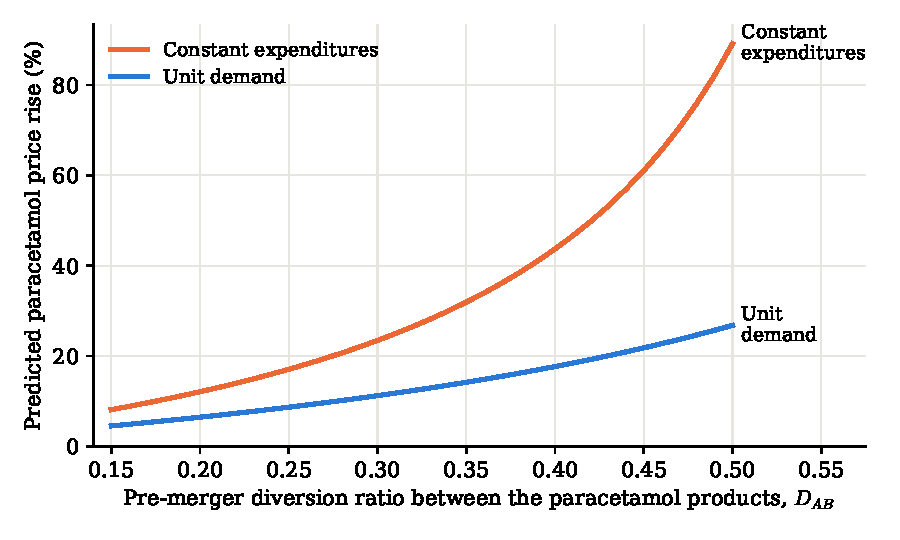
\includegraphics[width=0.78\textwidth]{figures/ch11/bv_curvature.pdf}
\caption{Predicted paracetamol price increase in the stylized calibration of \cref{tab:11-bvcurv}, against the
pre-merger diversion ratio between the two paracetamol products. Both versions match the same own elasticity
($-3$), diversion ratio and margins. The constant-expenditure version predicts 1.8 to 3.3 times the increase of
the unit-demand version.}
\label{fig:11-bvcurv}
\end{figure}

\Cref{tab:11-bvcurv} and \cref{fig:11-bvcurv} show the result. With identical first-order information the
constant-expenditure version predicts about twice the unit-demand increase at $D_{AB}=0.30$ and almost three times at
$D_{AB}=0.45$. Over the range shown the ratio lies between 1.8 and 3.3. Upward pricing pressure cannot distinguish
the two models, because it uses only first-order information. The simulation can, but only through an assumption
about curvature that pre-merger data barely constrain. The calibration also reproduces the second pattern of
Table 6. Rival price effects are below 1\% in both versions, because nested logit with substance nests diverts little
demand from paracetamol to each rival substance.

\casehead{Robustness} The working paper reports sensitivity checks run during and after the review
\citep[Sections 4.1 and 4.2]{BjornerstedtVerboven2013}. A potential market of 1.5, 4 or 6 times average sales, in
place of 2, gave similar results. A coarser product definition, with about 20 brand-form products per month instead
of 43, gave comparable findings. The full sample of 11,185 product-months gave the same conclusions as the
estimation sample. Adding sums of the pack sizes and doses of other products to the instruments left the unit-demand
results unchanged. Under constant expenditures it raised the elasticities and lowered the predicted price effects
somewhat, without changing the qualitative conclusions. Treating marketing as endogenous gave closely comparable
results. The reverse nesting order was rejected, as noted above.

\casehead{Interpretation} The study delivers three lessons. First, the constant-expenditure nested logit got the size
of the merging firms' price increase about right. It did so in the prediction made during the review, before the
outcome was known, and again in the published re-estimation. Second, the choice between specifications that fit the pre-merger data comparably
matters as much as the estimation itself. The unit-demand specifications implied implausibly elastic demand and low
margins, and they under-predicted the price increase by half or more. Third, the models missed how the effects were
distributed. They predicted very different increases for the two merging firms and small rival responses. The data
show similar increases for the two merging firms and increases of about 10 percent for some rivals.

Several explanations are possible. After the merger the merged firm cut its pack sizes from 30 to 20 tablets, as the
Swedish Medical Products Agency required. It lowered pack prices only slightly, for example from 41.5 to 38.5 kronor
for one of its best-selling products. The firms attributed the higher price per tablet to the cost of smaller packs. The authors
find this implausible, because ASA producers faced the same requirement without increases of similar size. The same
requirement may explain part of the ASA increase \citep[p.~29]{BjornerstedtVerboven2013}. The published version
considers a plausible post-merger cost increase and partial collusion as supply-side explanations
\citep[abstract]{BjornerstedtVerboven2016}. Rivals may have coordinated on higher prices after the merger, a
coordinated effect that a Bertrand model rules out (\cref{sec:11-millercoors}). The deregulation of pharmacies also
changed retail conditions in the same period. Finally, GSK was the acquirer and may have favored its own brands
after the merger. That would fit the small loss in its share (p.~32).

\casehead{Critiques and related validation studies} A single merger is a small sample for grading a method. The
retrospective benchmark rests on before-after comparisons of product-group prices, with rival controls whose prices
themselves moved. The change in pack sizes at the time of the merger further complicates the comparison of prices per
tablet. The predictions condition on the demand model's nest structure, which fixes how much substitution toward
rival substances is possible. Simulations that impose small cross-substance diversion will under-predict rivals'
responses whatever the curvature. \citet[p.~231]{AskerNocke2021} list four studies that grade merger simulations
with ex post evaluations: \citet{Peters2006}, \citet{Weinberg2011}, \citet{WeinbergHosken2013} and the present paper.
They reach mixed conclusions. \citet[pp.~627--628]{Peters2006} simulates five airline mergers completed between
August 1986 and November 1987. Standard simulations do not generally forecast the observed fare changes accurately.
Unobserved supply-side changes account for most of the gap in almost every case (p.~645). Peters concludes that
departures from the assumed model of conduct play an important role. \citet[p.~1584]{WeinbergHosken2013} simulate
two of the mergers of \cref{sec:11-ah}, Pennzoil and Quaker State in motor oil and Aurora and Log Cabin in syrup. For
motor oil the simulated increases are typically below 5 percent, against direct estimates of 4 to 8 percent. For
syrup the simulations typically predict 5 to 20 percent, while the merger had little effect on consumer prices.
\citet{AshenfelterHosken2010} find that the cereal simulation of \citet{Nevo2000b} predicted the wrong products to
rise in price (\cref{sec:11-ah}). \citet{Houde2012} compares a spatial simulation with a DiD estimate of the same
gasoline transaction (\cref{sec:11-beyond}).

\casehead{Contribution} The paper is one of the few direct tests of merger simulation as used by competition
authorities. It shows that simulations can predict the main effect of a merger when demand curvature is allowed to
be realistic. It also introduced the constant-expenditure nested logit, a tractable alternative to unit demand for
frequently purchased goods. Unit demand, the common default in discrete-choice models, can lead to large under-predictions even
when the model fits the pre-merger data. Retrospectives such as those in \cref{sec:11-retro} are therefore part of
the toolkit for choosing among prospective models.
